% Generated by scripts/narmyn/attention/build_evidence.py. Preamble: \usepackage{array,booktabs,longtable,float,graphicx} (array before longtable).
\section{Evidence: experiments and how each setting was reached}

{\scriptsize\setlength{\tabcolsep}{3pt}
\begin{longtable}{>{\raggedright\arraybackslash}p{1.40cm}>{\raggedright\arraybackslash}p{2.22cm}>{\raggedright\arraybackslash}p{2.46cm}>{\raggedright\arraybackslash}p{2.00cm}rr>{\raggedright\arraybackslash}p{2.88cm}}
\caption{Every experiment run so far}\label{tab:ledger}\\
\toprule
ID & Experiment & Dataset & Status & Configurations & Best mIoU & Decision /\allowbreak{} role \\
\midrule
\endfirsthead
\toprule
ID & Experiment & Dataset & Status & Configurations & Best mIoU & Decision /\allowbreak{} role \\
\midrule
\endhead
B1 & CA time windows and resolutions & VOC-Sim dev subset (99 images, 4 classes; inside the 490) & exploratory, in-sample & 11 & 0.7095 & first look at time and resolution \\
B2 & Single and leave-out CA layers & VOC-Sim dev subset (99 images, 4 classes; inside the 490) & exploratory, in-sample & 24 & 0.7232 & layer screening \\
B3 & Joint time x resolution & VOC-Sim dev subset (99 images, 4 classes; inside the 490) & exploratory, in-sample & 21 & 0.7095 & interaction check \\
B4 & Exhaustive CA layer subsets & VOC-Sim dev subset (99 images, 4 classes; inside the 490) & exploratory, in-sample & 17 & 0.7409 & chose BEST\_\allowbreak{}12 = layers \{0,2,5,6,7,9,10,11,12,13,14,15\} \\
B5 & Threshold x normalization & VOC-Sim dev subset (99 images, 4 classes; inside the 490) & exploratory, in-sample & 153 & 0.7439 & chose percentile 1-99 and threshold 0.45 \\
B6 & Stage-1 suite (heads, time-layer, fusion, cleanup) & VOC-Sim dev subset (99 images, 4 classes; inside the 490) & exploratory, in-sample & 590 & 0.7691 & chose the fixed top-4 CA heads per layer \\
B7 & Self-attention screens and progressive SA & VOC-Sim dev subset (99 images, 4 classes; inside the 490) & exploratory, in-sample & 5320 & 0.8355 & first evidence that SA propagation helps \\
B8 & Full streaming ablations & VOC-Sim (490 images, 20 classes) & exploratory, in-sample (choices from B1-B7 frozen) & 6261 & 0.7777 & SA at U3.2 (64x64), 4 passes: 0.7777 \\
B9 & Focused SA follow-up & VOC-Sim (490 images, 20 classes) & exploratory, in-sample & 1632 & 0.7922 & top-4-head seed, 2 passes, t=0.45: 0.7922 \\
B10 & Joint SA head x time x passes x threshold & VOC-Sim (490 images, 20 classes) & exploratory, in-sample & 4680 & 0.7997 & final method: 4 passes, heads \{0,1,2,4,5,6\}, calls 15-30, t=0.45, 1\% cleanup: 0.7997 \\
B11 & Component ablation of the final method & VOC-Sim (490 images, 20 classes); COCO-Cap (707 images, 20 classes) & exploratory (COCO untuned) & 18 & 0.7999 & SA propagation is the largest component \\
B12 & COCO-Cap generalization of the final method & COCO-Cap (707 images, 20 classes) & untuned transfer & 6 & 0.6080 & 0.5719 -> 0.6080 \\
B13 & Revised system (1 pass, all 16 CA layers) and its ablation & VOC-Sim (490 images, 20 classes); COCO-Cap (707 images, 20 classes) & exploratory; informed by COCO-Cap & 14 & 0.7837 & revised system: VOC 0.7824, COCO 0.6322 \\
B14 & CA call windows with all SA heads & VOC-Sim (490 images, 20 classes); COCO-Cap (707 images, 20 classes) & exploratory & 4 & 0.7811 & no gain over all calls \\
B15 & Clean CA-only screens (pre-sync) & VOC-Sim (490 images, 20 classes) & exploratory, in-sample; audited, superseded by A1 & 1573 & 0.6968 & ratified as correct; re-run with folds as A1 \\
B16 & OVAM released masks & VOC-Sim (490 images, 20 classes) & reference (authors' masks) & 3 & 0.8247 & 0.7036 /\allowbreak{} 0.8247 /\allowbreak{} 0.6616 \\
B17 & OVAM optimized token and DenseCRF on the final method & VOC-Sim (490 images, 20 classes); COCO-Cap (707 images, 20 classes) & exploratory; nothing selected & 32 & 0.8553 & token + DenseCRF: VOC 0.8525, COCO 0.6612 \\
A1 & Controlled CA package B: CA-L, CA-H, CA-A & VOC-Sim (490 images, 20 classes) & controlled, 5-fold cross-validated & 65961 & 0.6923 & CA-L drop modules 10-11; CA-H drop head 1; CA-A keep reference (CA-C pending) \\
A2 & Controlled CA package A: CA-T, CA-R (Codex) & VOC-Sim (490 images, 20 classes) & controlled, 5-fold cross-validated & 1279 & 0.6957 & CA-T keep all calls; CA-R keep 8+16+64 (drop 32x32) (CA-C pending) \\
\bottomrule
\end{longtable}}

\begin{table}[H]\centering\scriptsize\setlength{\tabcolsep}{3pt}
\begin{tabular}{>{\raggedright\arraybackslash}p{1.56cm}>{\raggedright\arraybackslash}p{2.59cm}>{\raggedright\arraybackslash}p{2.88cm}>{\raggedright\arraybackslash}p{1.75cm}>{\raggedright\arraybackslash}p{1.64cm}>{\raggedright\arraybackslash}p{3.73cm}}
\toprule
Setting & Value used so far & Chosen in & Images used to choose & Evidence & Controlled status \\
\midrule
CA layers & 12 of 16 (drop 1, 3, 4, 8) & B4 exhaustive search & 99 dev images & ledger B4; Fig. a1\_\allowbreak{}exhaustive & A1 CA-L (CV): keep all but modules 10, 11 instead; awaiting CA-C \\
CA heads & fixed top-4 per layer & B6 stage-1 suite & 99 dev images & ledger B6 & A1 CA-H (CV): drop head 1 in every module; awaiting CA-C \\
CA attribution & OVAM: unconditional query, unpadded softmax, first piece & inherited from OVAM & --- & Table a1\_\allowbreak{}ca\_\allowbreak{}a & A1 CA-A (CV): reference (conditional, padded, all pieces) kept; OVAM's cell is $-$0.0156 CA-only \\
CA calls & all 31 (0--30) & B1/\allowbreak{}B8 windows; B14 & 99 dev /\allowbreak{} 490 & ledger B1, B8, B14 & A2 CA-T (Codex), pending \\
CA normalization, threshold & percentile 1--99, $\geq$ 0.45 & B5 & 99 dev images & ledger B5 & protocol fixes min--max, 0.45 for the CA phase \\
SA module & U3.2 (up\_\allowbreak{}blocks.3.attentions.2 attn1, 64$\times$64) & B8 SA screens & 490 (in-sample) & ledger B8 & SA-L (Claude) after CA freeze \\
SA passes & 4 (revised: 1) & B10; revised from B11/\allowbreak{}B13 & 490; 1-pass informed by COCO-Cap & Fig. b\_\allowbreak{}joint\_\allowbreak{}passes\_\allowbreak{}time & after SA freeze \\
SA heads & \{0,1,2,4,5,6\} & B10 & 490 (in-sample) & Fig. b\_\allowbreak{}joint\_\allowbreak{}heads\_\allowbreak{}threshold & SA-H (Claude) after CA freeze \\
SA calls & 15--30 & B10 & 490 (in-sample) & Fig. b\_\allowbreak{}joint\_\allowbreak{}passes\_\allowbreak{}time & SA-T (Codex) after CA freeze \\
Mask threshold & 0.45 & B5, B9, B10 & 99 dev /\allowbreak{} 490 & Fig. b\_\allowbreak{}joint\_\allowbreak{}heads\_\allowbreak{}threshold & fixed at 0.45; 0.35/\allowbreak{}0.55 as diagnostics \\
Cleanup & remove components < 1\% & B10 & 490 (in-sample) & Table b\_\allowbreak{}component\_\allowbreak{}ablations & deferred phase \\
DenseCRF & not in the final method & B17 (nothing selected) & --- & Table b\_\allowbreak{}token\_\allowbreak{}crf & deferred phase \\
Optimized token & not in the final method & B17 (nothing selected; tokens trained by OVAM on separate images) & --- & Table b\_\allowbreak{}token\_\allowbreak{}crf & deferred phase \\
\bottomrule
\end{tabular}
\caption{Where each setting of the method came from}\label{tab:decision_trail}
\end{table}

\begin{table}[H]\centering\scriptsize\setlength{\tabcolsep}{3pt}
\begin{tabular}{>{\raggedright\arraybackslash}p{1.40cm}>{\raggedright\arraybackslash}p{1.40cm}>{\raggedright\arraybackslash}p{1.40cm}>{\raggedright\arraybackslash}p{1.40cm}rrr>{\raggedright\arraybackslash}p{1.40cm}>{\raggedright\arraybackslash}p{1.40cm}>{\raggedright\arraybackslash}p{1.40cm}}
\toprule
Screen & Package & Reference & Vote winner (votes) & OOF mIoU reference & OOF mIoU choice & OOF gain & Paired $\Delta$ image IoU [95\% CI] & $\Delta$ mIoU @0.35 /\allowbreak{} 0.45 /\allowbreak{} 0.55 & Outcome \\
\midrule
CA-T & A (Codex) & time/\allowbreak{}all\_\allowbreak{}00\_\allowbreak{}30 & time/\allowbreak{}all\_\allowbreak{}00\_\allowbreak{}30 (5/\allowbreak{}5) & 0.6661 & 0.6661 & 0.0000 & +0.0000 [+0.0000, +0.0000] & +0.0000 /\allowbreak{} +0.0000 /\allowbreak{} +0.0000 & reference won the fold vote \\
CA-R & A (Codex) & resolution/\allowbreak{}r8\_\allowbreak{}r16\_\allowbreak{}r32\_\allowbreak{}r64 & resolution/\allowbreak{}r8\_\allowbreak{}r16\_\allowbreak{}r64 (5/\allowbreak{}5) & 0.6661 & 0.6957 & 0.0296 & +0.0211 [+0.0139, +0.0286] & +0.0009 /\allowbreak{} +0.0296 /\allowbreak{} +0.0442 & fold vote and OOF guard passed \\
CA-L & B (Claude) & L/\allowbreak{}all\_\allowbreak{}16 & L/\allowbreak{}leave2\_\allowbreak{}10\_\allowbreak{}11 (5/\allowbreak{}5) & 0.6661 & 0.6923 & 0.0262 & +0.0209 [+0.0155, +0.0265] & -0.0021 /\allowbreak{} +0.0262 /\allowbreak{} +0.0501 & fold vote and OOF guard passed \\
CA-H & B (Claude) & H/\allowbreak{}0\_\allowbreak{}1\_\allowbreak{}2\_\allowbreak{}3\_\allowbreak{}4\_\allowbreak{}5\_\allowbreak{}6\_\allowbreak{}7 & H/\allowbreak{}0\_\allowbreak{}2\_\allowbreak{}3\_\allowbreak{}4\_\allowbreak{}5\_\allowbreak{}6\_\allowbreak{}7 (4/\allowbreak{}5) & 0.6661 & 0.6741 & 0.0080 & +0.0089 [+0.0047, +0.0131] & -0.0002 /\allowbreak{} +0.0104 /\allowbreak{} +0.0193 & fold vote and OOF guard passed \\
CA-A & B (Claude) & A/\allowbreak{}cond\_\allowbreak{}padded\_\allowbreak{}all & A/\allowbreak{}cond\_\allowbreak{}padded\_\allowbreak{}all (5/\allowbreak{}5) & 0.6661 & 0.6661 & 0.0000 & +0.0000 [+0.0000, +0.0000] & +0.0000 /\allowbreak{} +0.0000 /\allowbreak{} +0.0000 & reference won the fold vote \\
CA-C & C (Claude) & C/\allowbreak{}reference & C/\allowbreak{}R (4/\allowbreak{}5) & 0.6653 & 0.6914 & 0.0260 & +0.0217 [+0.0145, +0.0293] & +0.0010 /\allowbreak{} +0.0303 /\allowbreak{} +0.0447 & fold vote and OOF guard passed \\
\bottomrule
\end{tabular}
\caption{Controlled CA screens (VOC-Sim, 5 folds, selection at threshold 0.45). The single-axis screens promote candidates; only the combined confirmation (CA-C) freezes the CA.}\label{tab:a_cv_summary}
\end{table}

\begin{table}[H]\centering\scriptsize\setlength{\tabcolsep}{3pt}
\begin{tabular}{>{\raggedright\arraybackslash}p{4.00cm}rrrrr>{\raggedright\arraybackslash}p{1.77cm}}
\toprule
Configuration & mIoU@0.45 & $\Delta$ vs reference & mIoU@0.35 & mIoU@0.55 & Mean AP & Fold votes \\
\midrule
reference (16 modules, 8 heads) & 0.6653 & 0.0000 & 0.7057 & 0.5430 & 0.9218 & 0/\allowbreak{}5 \\
CA-R: without 32$\times$32 (11 modules) & 0.6956 & 0.0303 & 0.7067 & 0.5877 & 0.9131 & 4/\allowbreak{}5 \\
CA-L: without modules 10, 11 & 0.6921 & 0.0267 & 0.7035 & 0.5938 & 0.9201 & 1/\allowbreak{}5 \\
CA-H: without head 1 & 0.6761 & 0.0108 & 0.7056 & 0.5623 & 0.9205 & 0/\allowbreak{}5 \\
CA-R + CA-H & 0.6960 & 0.0307 & 0.7058 & 0.5879 & 0.9127 & 0/\allowbreak{}5 \\
CA-L + CA-H & 0.6924 & 0.0270 & 0.7020 & 0.5948 & 0.9190 & 0/\allowbreak{}5 \\
\bottomrule
\end{tabular}
\caption{CA-C: the combined confirmation (one run, in-sample values; fold votes from the 5-fold selection)}\label{tab:a3_ca_c}
\end{table}

\begin{table}[H]\centering\scriptsize\setlength{\tabcolsep}{3pt}
\begin{tabular}{>{\raggedright\arraybackslash}p{4.83cm}rr>{\raggedright\arraybackslash}p{5.99cm}}
\toprule
Combined candidate & mIoU@0.45 & $\Delta$ vs combined & Reading \\
\midrule
combined CA-R + CA-H & 0.6960 & 0.0000 & --- \\
without CA-R (= CA-L + CA-H) & 0.6924 & -0.0036 & CA-R contributes \\
without CA-H (= CA-R alone) & 0.6956 & -0.0004 & within the 0.002 tie: CA-H is not kept \\
without CA-L & 0.6960 & 0.0000 & CA-L is contained in CA-R \\
\bottomrule
\end{tabular}
\caption{CA-C leave-one-out of the combined candidate (in-sample)}\label{tab:a3_ca_c_loo}
\end{table}

\begin{table}[H]\centering\scriptsize\setlength{\tabcolsep}{3pt}
\begin{tabular}{r>{\raggedright\arraybackslash}p{1.40cm}rrrr}
\toprule
Held-out fold & Chosen on the other four & Train mIoU chosen & Train mIoU reference & Held-out mIoU chosen & Held-out mIoU reference \\
\midrule
0 & CA-R: without 32$\times$32 (11 modules) & 0.6967 & 0.6644 & 0.6905 & 0.6708 \\
1 & CA-R: without 32$\times$32 (11 modules) & 0.6912 & 0.6610 & 0.7116 & 0.6827 \\
2 & CA-R: without 32$\times$32 (11 modules) & 0.6957 & 0.6641 & 0.6973 & 0.6714 \\
3 & CA-R: without 32$\times$32 (11 modules) & 0.6975 & 0.6661 & 0.6868 & 0.6676 \\
4 & CA-L: without modules 10, 11 & 0.6977 & 0.6715 & 0.6702 & 0.6429 \\
\bottomrule
\end{tabular}
\caption{CA-C: the choice made on each set of four folds and its held-out score}\label{tab:a3_ca_c_folds}
\end{table}

\begin{table}[H]\centering\scriptsize\setlength{\tabcolsep}{3pt}
\begin{tabular}{>{\raggedright\arraybackslash}p{3.22cm}rrrrrr}
\toprule
Configuration & mIoU@0.45 & $\Delta$ vs reference & mIoU@0.35 & mIoU@0.55 & Mean AP & SD across folds \\
\midrule
all 00 30 & 0.6661 & 0.0000 & 0.7059 & 0.5434 & 0.9218 & 0.0133 \\
window 00 04 & 0.5622 & -0.1039 & 0.5373 & 0.5393 & 0.8041 & 0.0168 \\
window 05 09 & 0.6469 & -0.0192 & 0.6742 & 0.5465 & 0.8976 & 0.0131 \\
window 10 14 & 0.6224 & -0.0437 & 0.6943 & 0.4670 & 0.9086 & 0.0122 \\
window 15 20 & 0.5796 & -0.0865 & 0.6887 & 0.4031 & 0.9048 & 0.0096 \\
window 21 25 & 0.5224 & -0.1437 & 0.6623 & 0.3409 & 0.8979 & 0.0122 \\
window 26 30 & 0.4524 & -0.2137 & 0.6159 & 0.2789 & 0.8955 & 0.0081 \\
trailing 05 30 & 0.6320 & -0.0341 & 0.7077 & 0.4803 & 0.9206 & 0.0106 \\
trailing 10 30 & 0.5893 & -0.0768 & 0.6941 & 0.4209 & 0.9132 & 0.0097 \\
trailing 15 30 & 0.5491 & -0.1170 & 0.6767 & 0.3730 & 0.9064 & 0.0114 \\
trailing 21 30 & 0.4998 & -0.1663 & 0.6509 & 0.3215 & 0.8997 & 0.0108 \\
trailing 26 30 & 0.4524 & -0.2137 & 0.6159 & 0.2789 & 0.8955 & 0.0081 \\
cumulative 00 04 & 0.5622 & -0.1039 & 0.5373 & 0.5393 & 0.8041 & 0.0168 \\
cumulative 00 09 & 0.6387 & -0.0274 & 0.6137 & 0.5860 & 0.8755 & 0.0153 \\
cumulative 00 14 & 0.6668 & 0.0007 & 0.6617 & 0.5899 & 0.9034 & 0.0134 \\
cumulative 00 20 & 0.6752 & 0.0091 & 0.6886 & 0.5763 & 0.9157 & 0.0136 \\
cumulative 00 25 & 0.6727 & 0.0066 & 0.7001 & 0.5601 & 0.9198 & 0.0138 \\
\bottomrule
\end{tabular}
\caption{CA-T: call windows (in-sample; all 79 configurations, including every single call and leave-one-call-out, in controlled\_\allowbreak{}ca\_\allowbreak{}package\_\allowbreak{}a.csv)}\label{tab:a2_ca_t}
\end{table}

\begin{table}[H]\centering\scriptsize\setlength{\tabcolsep}{3pt}
\begin{tabular}{>{\raggedright\arraybackslash}p{2.87cm}rrrrrr}
\toprule
Configuration & mIoU@0.45 & $\Delta$ vs reference & mIoU@0.35 & mIoU@0.55 & Mean AP & SD across folds \\
\midrule
8+16+64 & 0.6957 & 0.0296 & 0.7068 & 0.5876 & 0.9131 & 0.0092 \\
8+16 & 0.6933 & 0.0272 & 0.7148 & 0.5942 & 0.9171 & 0.0094 \\
8+16+32+64 & 0.6661 & 0.0000 & 0.7059 & 0.5434 & 0.9218 & 0.0133 \\
8+16+32 & 0.6562 & -0.0099 & 0.7082 & 0.5323 & 0.9240 & 0.0112 \\
16 & 0.6489 & -0.0172 & 0.7099 & 0.5086 & 0.9059 & 0.0142 \\
16+64 & 0.6449 & -0.0212 & 0.6906 & 0.4925 & 0.8902 & 0.0130 \\
16+32+64 & 0.6138 & -0.0523 & 0.6849 & 0.4590 & 0.9031 & 0.0125 \\
16+32 & 0.6004 & -0.0657 & 0.6877 & 0.4461 & 0.9092 & 0.0127 \\
8+32+64 & 0.5632 & -0.1029 & 0.6403 & 0.4193 & 0.8929 & 0.0093 \\
8 & 0.5626 & -0.1035 & 0.6021 & 0.4787 & 0.8462 & 0.0084 \\
8+64 & 0.5435 & -0.1226 & 0.6001 & 0.4002 & 0.8307 & 0.0037 \\
8+32 & 0.5328 & -0.1333 & 0.6212 & 0.4106 & 0.8969 & 0.0089 \\
32+64 & 0.3693 & -0.2968 & 0.5075 & 0.2045 & 0.8043 & 0.0109 \\
32 & 0.2995 & -0.3666 & 0.4422 & 0.1740 & 0.8221 & 0.0115 \\
64 & 0.1734 & -0.4927 & 0.3285 & 0.0631 & 0.5604 & 0.0084 \\
\bottomrule
\end{tabular}
\caption{CA-R: all 15 resolution subsets (in-sample; reference 8+16+32+64)}\label{tab:a2_ca_r}
\end{table}

\begin{table}[H]\centering\scriptsize\setlength{\tabcolsep}{3pt}
\begin{tabular}{>{\raggedright\arraybackslash}p{3.73cm}rrrrrr}
\toprule
Configuration & mIoU@0.45 & $\Delta$ vs all 16 & mIoU@0.35 & mIoU@0.55 & Mean AP & SD across folds \\
\midrule
without 10 U2.0 \& 11 U2.1 & 0.6923 & 0.0262 & 0.7036 & 0.5937 & 0.9201 & 0.0132 \\
without 10 U2.0 \& 12 U2.2 & 0.6870 & 0.0209 & 0.7060 & 0.5832 & 0.9199 & 0.0124 \\
without 11 U2.1 \& 12 U2.2 & 0.6860 & 0.0200 & 0.7016 & 0.5825 & 0.9179 & 0.0147 \\
without 11 U2.1 \& 14 U3.1 & 0.6852 & 0.0191 & 0.7076 & 0.5771 & 0.9220 & 0.0156 \\
without 11 U2.1 \& 15 U3.2 & 0.6851 & 0.0190 & 0.7062 & 0.5756 & 0.9207 & 0.0154 \\
without 10 U2.0 \& 14 U3.1 & 0.6831 & 0.0170 & 0.7088 & 0.5743 & 0.9236 & 0.0131 \\
without 10 U2.0 \& 15 U3.2 & 0.6828 & 0.0168 & 0.7070 & 0.5731 & 0.9222 & 0.0134 \\
without 09 U1.2 \& 11 U2.1 & 0.6826 & 0.0165 & 0.7026 & 0.5725 & 0.9183 & 0.0151 \\
without 09 U1.2 \& 10 U2.0 & 0.6806 & 0.0145 & 0.7037 & 0.5697 & 0.9200 & 0.0131 \\
without 03 D1.1 \& 11 U2.1 & 0.6803 & 0.0142 & 0.7078 & 0.5678 & 0.9213 & 0.0148 \\
\bottomrule
\end{tabular}
\caption{CA-L: the ten best leave-two-out configurations (in-sample)}\label{tab:a1_ca_l_leave2}
\end{table}

\begin{table}[H]\centering\scriptsize\setlength{\tabcolsep}{3pt}
\begin{tabular}{rrrr>{\raggedright\arraybackslash}p{3.82cm}}
\toprule
Head & Alone & All but this head & $\Delta$ vs all 8 & Folds retaining it \\
\midrule
0 & 0.2557 & 0.6484 & -0.0177 & 5/\allowbreak{}5 \\
1 & 0.0975 & 0.6765 & 0.0104 & 1/\allowbreak{}5 \\
2 & 0.3638 & 0.6471 & -0.0190 & 5/\allowbreak{}5 \\
3 & 0.3556 & 0.6549 & -0.0112 & 5/\allowbreak{}5 \\
4 & 0.4344 & 0.6448 & -0.0213 & 5/\allowbreak{}5 \\
5 & 0.4179 & 0.6516 & -0.0144 & 5/\allowbreak{}5 \\
6 & 0.3208 & 0.6456 & -0.0205 & 5/\allowbreak{}5 \\
7 & 0.3165 & 0.6581 & -0.0080 & 5/\allowbreak{}5 \\
\bottomrule
\end{tabular}
\caption{CA-H: each head alone and leave-one-out (in-sample mIoU at 0.45), and fold retention}\label{tab:a1_ca_h_heads}
\end{table}

\begin{table}[H]\centering\scriptsize\setlength{\tabcolsep}{3pt}
\begin{tabular}{r>{\raggedright\arraybackslash}p{1.73cm}>{\raggedright\arraybackslash}p{3.25cm}r}
\toprule
Round & Removed & Heads left & mIoU@0.45 \\
\midrule
0 & --- & 0 1 2 3 4 5 6 7 & 0.6661 \\
1 & 1 & 0 2 3 4 5 6 7 & 0.6765 \\
2 & 5 & 0 2 3 4 6 7 & 0.6718 \\
3 & 7 & 0 2 3 4 6 & 0.6609 \\
4 & 0 & 2 3 4 6 & 0.6388 \\
5 & 2 & 3 4 6 & 0.6005 \\
6 & 6 & 3 4 & 0.5444 \\
7 & 3 & 4 & 0.4344 \\
\bottomrule
\end{tabular}
\caption{CA-H: greedy backward elimination (in-sample)}\label{tab:a1_ca_h_greedy}
\end{table}

\begin{table}[H]\centering\scriptsize\setlength{\tabcolsep}{3pt}
\begin{tabular}{>{\raggedright\arraybackslash}p{3.25cm}rrrrrr}
\toprule
Head subset & Heads & mIoU@0.45 & $\Delta$ vs all 8 & mIoU@0.35 & mIoU@0.55 & Mean AP \\
\midrule
0 2 3 4 5 6 7 & 7 & 0.6765 & 0.0104 & 0.7055 & 0.5629 & 0.9206 \\
0 2 3 4 6 7 & 6 & 0.6718 & 0.0058 & 0.7110 & 0.5406 & 0.9121 \\
0 2 3 4 5 6 & 6 & 0.6676 & 0.0015 & 0.7044 & 0.5514 & 0.9138 \\
0 1 2 3 4 5 6 7 & 8 & 0.6661 & -0.0000 & 0.7057 & 0.5435 & 0.9218 \\
0 2 3 4 5 7 & 6 & 0.6629 & -0.0031 & 0.7038 & 0.5377 & 0.9173 \\
0 3 4 5 6 7 & 6 & 0.6626 & -0.0035 & 0.6928 & 0.5373 & 0.9084 \\
2 3 4 5 6 7 & 6 & 0.6625 & -0.0035 & 0.7035 & 0.5405 & 0.9236 \\
0 2 4 5 6 7 & 6 & 0.6615 & -0.0046 & 0.7011 & 0.5424 & 0.9140 \\
0 2 3 4 6 & 5 & 0.6609 & -0.0052 & 0.7095 & 0.5248 & 0.9005 \\
0 1 2 3 4 5 6 & 7 & 0.6581 & -0.0080 & 0.7044 & 0.5371 & 0.9167 \\
0 2 3 5 6 7 & 6 & 0.6571 & -0.0090 & 0.6935 & 0.5325 & 0.9092 \\
2 3 4 5 6 & 5 & 0.6564 & -0.0097 & 0.7032 & 0.5324 & 0.9173 \\
0 1 2 4 5 6 7 & 7 & 0.6549 & -0.0112 & 0.7021 & 0.5274 & 0.9155 \\
0 2 3 4 5 & 5 & 0.6541 & -0.0120 & 0.7022 & 0.5275 & 0.9137 \\
0 1 2 3 4 6 7 & 7 & 0.6516 & -0.0144 & 0.7059 & 0.5060 & 0.9142 \\
\bottomrule
\end{tabular}
\caption{CA-H: the 15 best of 255 head subsets (in-sample; all 255 in controlled\_\allowbreak{}ca\_\allowbreak{}package\_\allowbreak{}b.csv)}\label{tab:a1_ca_h_top}
\end{table}

\begin{table}[H]\centering\scriptsize\setlength{\tabcolsep}{3pt}
\begin{tabular}{>{\raggedright\arraybackslash}p{2.09cm}>{\raggedright\arraybackslash}p{1.49cm}>{\raggedright\arraybackslash}p{1.98cm}rrrrr}
\toprule
Query branch & Softmax & Class pieces & mIoU@0.45 & $\Delta$ vs reference & mIoU@0.35 & mIoU@0.55 & Mean AP \\
\midrule
conditional & unpadded & all & 0.6678 & 0.0018 & 0.7054 & 0.5480 & 0.9245 \\
conditional & padded & all & 0.6661 & 0.0000 & 0.7057 & 0.5435 & 0.9218 \\
unconditional & padded & all & 0.6612 & -0.0048 & 0.6992 & 0.5489 & 0.9222 \\
unconditional & unpadded & all & 0.6610 & -0.0050 & 0.6986 & 0.5506 & 0.9241 \\
conditional & unpadded & last & 0.6597 & -0.0063 & 0.6998 & 0.5414 & 0.9246 \\
conditional & padded & last & 0.6579 & -0.0082 & 0.7000 & 0.5365 & 0.9219 \\
unconditional & padded & last & 0.6541 & -0.0119 & 0.6938 & 0.5436 & 0.9223 \\
unconditional & unpadded & last & 0.6539 & -0.0122 & 0.6935 & 0.5454 & 0.9243 \\
unconditional & unpadded & first & 0.6505 & -0.0156 & 0.6970 & 0.5252 & 0.9127 \\
conditional & unpadded & first & 0.6479 & -0.0182 & 0.6962 & 0.5172 & 0.9107 \\
unconditional & padded & first & 0.6474 & -0.0187 & 0.6967 & 0.5199 & 0.9106 \\
conditional & padded & first & 0.6451 & -0.0210 & 0.6953 & 0.5112 & 0.9080 \\
\bottomrule
\end{tabular}
\caption{CA-A: the 12 attribution conventions (in-sample; reference = conditional, padded, all)}\label{tab:a1_ca_a}
\end{table}

\begin{table}[H]\centering\scriptsize\setlength{\tabcolsep}{3pt}
\begin{tabular}{>{\raggedright\arraybackslash}p{4.26cm}rrrrr>{\raggedright\arraybackslash}p{1.51cm}}
\toprule
Configuration & mIoU@0.45 & $\Delta$ vs reference & mIoU@0.35 & mIoU@0.55 & Mean AP & Fold votes \\
\midrule
reference (16 SA modules, 31 calls, 8 heads) & 0.7556 & 0.0000 & 0.7213 & 0.7466 & 0.9536 & 0/\allowbreak{}5 \\
T: call 30 only & 0.7710 & 0.0153 & 0.7465 & 0.7457 & 0.9551 & 0/\allowbreak{}5 \\
R: resolutions 8+64 & 0.7676 & 0.0119 & 0.7414 & 0.7399 & 0.9542 & 0/\allowbreak{}5 \\
L: module 15 only (U3.2) & 0.7887 & 0.0330 & 0.7691 & 0.7532 & 0.9560 & 5/\allowbreak{}5 \\
H: heads 1, 4, 6 & 0.7613 & 0.0057 & 0.7295 & 0.7470 & 0.9552 & 0/\allowbreak{}5 \\
T + R & 0.7749 & 0.0193 & 0.7659 & 0.7244 & 0.9517 & 0/\allowbreak{}5 \\
T + L & 0.7820 & 0.0264 & 0.7704 & 0.7260 & 0.9474 & 0/\allowbreak{}5 \\
T + H & 0.7732 & 0.0175 & 0.7534 & 0.7412 & 0.9563 & 0/\allowbreak{}5 \\
R + H & 0.7656 & 0.0099 & 0.7389 & 0.7343 & 0.9534 & 0/\allowbreak{}5 \\
L + H & 0.7871 & 0.0314 & 0.7637 & 0.7554 & 0.9587 & 0/\allowbreak{}5 \\
T + R + H & 0.7692 & 0.0136 & 0.7669 & 0.7098 & 0.9512 & 0/\allowbreak{}5 \\
T + L + H & 0.7825 & 0.0268 & 0.7658 & 0.7330 & 0.9514 & 0/\allowbreak{}5 \\
\bottomrule
\end{tabular}
\caption{SA-C: the combined confirmation (one run, in-sample values; fold votes from the 5-fold selection)}\label{tab:a6_sa_c}
\end{table}

\begin{table}[H]\centering\scriptsize\setlength{\tabcolsep}{3pt}
\begin{tabular}{>{\raggedright\arraybackslash}p{3.06cm}>{\raggedright\arraybackslash}p{2.11cm}>{\raggedright\arraybackslash}p{1.73cm}r}
\toprule
Component & With & Without & $\Delta$ mIoU@0.45 \\
\midrule
T within T+L+H & T + L + H & L + H & -0.0046 \\
L within T+L+H & T + L + H & T + H & 0.0093 \\
H within T+L+H & T + L + H & T + L & 0.0005 \\
R within T+R+H & T + R + H & T + H & -0.0040 \\
\bottomrule
\end{tabular}
\caption{SA-C: removing one component from the full combination (in-sample)}\label{tab:a6_sa_c_components}
\end{table}

\begin{table}[H]\centering\scriptsize\setlength{\tabcolsep}{3pt}
\begin{tabular}{r>{\raggedright\arraybackslash}p{1.40cm}rrrr}
\toprule
Held-out fold & Chosen on the other four & Train mIoU chosen & Train mIoU reference & Held-out mIoU chosen & Held-out mIoU reference \\
\midrule
0 & L: module 15 only (U3.2) & 0.7892 & 0.7580 & 0.7892 & 0.7465 \\
1 & L: module 15 only (U3.2) & 0.7825 & 0.7490 & 0.8116 & 0.7780 \\
2 & L: module 15 only (U3.2) & 0.7899 & 0.7571 & 0.7869 & 0.7518 \\
3 & L: module 15 only (U3.2) & 0.7908 & 0.7578 & 0.7825 & 0.7460 \\
4 & L: module 15 only (U3.2) & 0.7910 & 0.7559 & 0.7757 & 0.7484 \\
\bottomrule
\end{tabular}
\caption{SA-C: the choice made on each set of four folds and its held-out score}\label{tab:a6_sa_c_folds}
\end{table}

\begin{table}[H]\centering\scriptsize\setlength{\tabcolsep}{3pt}
\begin{tabular}{>{\raggedright\arraybackslash}p{2.68cm}rrr}
\toprule
Class & Reference & Module 15 only & $\Delta$ \\
\midrule
chair & 0.5289 & 0.6503 & 0.1214 \\
aeroplane & 0.7309 & 0.8450 & 0.1141 \\
bicycle & 0.6788 & 0.7471 & 0.0683 \\
boat & 0.7638 & 0.8318 & 0.0680 \\
bird & 0.7859 & 0.8531 & 0.0673 \\
bottle & 0.8126 & 0.8665 & 0.0539 \\
horse & 0.8300 & 0.8696 & 0.0396 \\
motorbike & 0.8157 & 0.8527 & 0.0370 \\
dog & 0.8692 & 0.8960 & 0.0268 \\
car & 0.8152 & 0.8420 & 0.0268 \\
train & 0.6470 & 0.6697 & 0.0227 \\
sofa & 0.9230 & 0.9447 & 0.0217 \\
dining-table & 0.4511 & 0.4677 & 0.0166 \\
cow & 0.8055 & 0.8184 & 0.0129 \\
cat & 0.7688 & 0.7816 & 0.0127 \\
bus & 0.9064 & 0.9184 & 0.0120 \\
sheep & 0.7564 & 0.7660 & 0.0096 \\
potted-plant & 0.7064 & 0.7091 & 0.0027 \\
tv & 0.7953 & 0.7768 & -0.0184 \\
person & 0.7218 & 0.6664 & -0.0554 \\
\bottomrule
\end{tabular}
\caption{SA-C: per-class IoU of the selected SA configuration against the inclusive SA reference (threshold 0.45)}\label{tab:a6_sa_c_classes}
\end{table}

\begin{table}[H]\centering\scriptsize\setlength{\tabcolsep}{3pt}
\begin{tabular}{>{\raggedright\arraybackslash}p{3.22cm}rrrrrr}
\toprule
Configuration & mIoU@0.45 & $\Delta$ vs reference & mIoU@0.35 & mIoU@0.55 & Mean AP & SD across folds \\
\midrule
all 00 30 & 0.7556 & 0.0000 & 0.7213 & 0.7466 & 0.9536 & 0.0121 \\
window 00 04 & 0.6105 & -0.1452 & 0.5513 & 0.6432 & 0.8907 & 0.0175 \\
window 05 09 & 0.7290 & -0.0266 & 0.6893 & 0.7286 & 0.9424 & 0.0130 \\
window 10 14 & 0.7569 & 0.0012 & 0.7241 & 0.7470 & 0.9535 & 0.0118 \\
window 15 20 & 0.7636 & 0.0079 & 0.7354 & 0.7477 & 0.9548 & 0.0110 \\
window 21 25 & 0.7661 & 0.0105 & 0.7412 & 0.7453 & 0.9544 & 0.0100 \\
window 26 30 & 0.7687 & 0.0131 & 0.7447 & 0.7447 & 0.9545 & 0.0098 \\
trailing 05 30 & 0.7617 & 0.0060 & 0.7318 & 0.7473 & 0.9549 & 0.0114 \\
trailing 10 30 & 0.7650 & 0.0093 & 0.7376 & 0.7474 & 0.9552 & 0.0108 \\
trailing 15 30 & 0.7663 & 0.0107 & 0.7407 & 0.7465 & 0.9549 & 0.0103 \\
trailing 21 30 & 0.7675 & 0.0119 & 0.7432 & 0.7452 & 0.9545 & 0.0098 \\
trailing 26 30 & 0.7687 & 0.0131 & 0.7447 & 0.7447 & 0.9545 & 0.0098 \\
cumulative 00 04 & 0.6105 & -0.1452 & 0.5513 & 0.6432 & 0.8907 & 0.0175 \\
cumulative 00 09 & 0.6956 & -0.0600 & 0.6390 & 0.7114 & 0.9318 & 0.0151 \\
cumulative 00 14 & 0.7276 & -0.0280 & 0.6813 & 0.7337 & 0.9454 & 0.0136 \\
cumulative 00 20 & 0.7441 & -0.0116 & 0.7042 & 0.7429 & 0.9508 & 0.0132 \\
cumulative 00 25 & 0.7510 & -0.0046 & 0.7143 & 0.7454 & 0.9526 & 0.0126 \\
\bottomrule
\end{tabular}
\caption{SA-T: call windows (in-sample; all 79 configurations, including every single call and leave-one-call-out, in controlled\_\allowbreak{}sa\_\allowbreak{}package\_\allowbreak{}a.csv)}\label{tab:a5_sa_t}
\end{table}

\begin{table}[H]\centering\scriptsize\setlength{\tabcolsep}{3pt}
\begin{tabular}{>{\raggedright\arraybackslash}p{2.87cm}rrrrrr}
\toprule
Configuration & mIoU@0.45 & $\Delta$ vs reference & mIoU@0.35 & mIoU@0.55 & Mean AP & SD across folds \\
\midrule
64 & 0.7678 & 0.0121 & 0.7474 & 0.7309 & 0.9539 & 0.0124 \\
8+64 & 0.7676 & 0.0119 & 0.7414 & 0.7399 & 0.9542 & 0.0128 \\
32+64 & 0.7627 & 0.0070 & 0.7388 & 0.7369 & 0.9550 & 0.0125 \\
8+32+64 & 0.7619 & 0.0063 & 0.7356 & 0.7399 & 0.9549 & 0.0125 \\
16+64 & 0.7578 & 0.0021 & 0.7199 & 0.7507 & 0.9531 & 0.0120 \\
16+32+64 & 0.7568 & 0.0012 & 0.7237 & 0.7457 & 0.9538 & 0.0120 \\
8+16+32+64 & 0.7556 & 0.0000 & 0.7213 & 0.7466 & 0.9536 & 0.0121 \\
8+16+64 & 0.7554 & -0.0002 & 0.7158 & 0.7516 & 0.9529 & 0.0123 \\
32 & 0.7532 & -0.0024 & 0.7275 & 0.7353 & 0.9534 & 0.0119 \\
8+32 & 0.7510 & -0.0047 & 0.7214 & 0.7387 & 0.9528 & 0.0122 \\
16+32 & 0.7434 & -0.0123 & 0.7066 & 0.7426 & 0.9503 & 0.0113 \\
8+16+32 & 0.7413 & -0.0144 & 0.7033 & 0.7430 & 0.9499 & 0.0116 \\
16 & 0.7187 & -0.0370 & 0.6749 & 0.7352 & 0.9402 & 0.0108 \\
8+16 & 0.7156 & -0.0400 & 0.6706 & 0.7343 & 0.9399 & 0.0112 \\
8 & 0.6764 & -0.0793 & 0.6237 & 0.6992 & 0.9030 & 0.0137 \\
\bottomrule
\end{tabular}
\caption{SA-R: all 15 resolution subsets (in-sample; reference 8+16+32+64)}\label{tab:a5_sa_r}
\end{table}

\begin{table}[H]\centering\scriptsize\setlength{\tabcolsep}{3pt}
\begin{tabular}{>{\raggedright\arraybackslash}p{1.40cm}>{\raggedright\arraybackslash}p{1.40cm}>{\raggedright\arraybackslash}p{1.40cm}rrr>{\raggedright\arraybackslash}p{1.40cm}>{\raggedright\arraybackslash}p{1.40cm}>{\raggedright\arraybackslash}p{1.42cm}}
\toprule
Screen & Reference & Vote winner (votes) & OOF mIoU reference & OOF mIoU choice & OOF gain & Paired $\Delta$ image IoU [95\% CI] & $\Delta$ mIoU @0.35 /\allowbreak{} 0.45 /\allowbreak{} 0.55 & Outcome \\
\midrule
SA-L & SL/\allowbreak{}all\_\allowbreak{}16 & SL/\allowbreak{}single\_\allowbreak{}15 (5/\allowbreak{}5) & 0.7553 & 0.7884 & 0.0331 & +0.0417 [+0.0365, +0.0469] & +0.0477 /\allowbreak{} +0.0331 /\allowbreak{} +0.0068 & fold vote and OOF guard passed \\
SA-H & SH/\allowbreak{}0\_\allowbreak{}1\_\allowbreak{}2\_\allowbreak{}3\_\allowbreak{}4\_\allowbreak{}5\_\allowbreak{}6\_\allowbreak{}7 & SH/\allowbreak{}1\_\allowbreak{}4\_\allowbreak{}6 (5/\allowbreak{}5) & 0.7553 & 0.7610 & 0.0057 & +0.0065 [+0.0056, +0.0074] & +0.0083 /\allowbreak{} +0.0057 /\allowbreak{} +0.0004 & fold vote and OOF guard passed \\
\bottomrule
\end{tabular}
\caption{Controlled SA package B (frozen CA seed; VOC-Sim, 5 folds, selection at 0.45). SA-C combines these with SA-T/\allowbreak{}SA-R.}\label{tab:a4_cv_summary}
\end{table}

\begin{table}[H]\centering\scriptsize\setlength{\tabcolsep}{3pt}
\begin{tabular}{>{\raggedright\arraybackslash}p{5.47cm}rrrrr}
\toprule
Configuration & mIoU@0.45 & $\Delta$ vs SA reference & mIoU@0.35 & mIoU@0.55 & Mean AP \\
\midrule
frozen CA seed alone (no SA) & 0.6956 & -0.0597 & 0.7067 & 0.5877 & 0.9131 \\
SA reference: all 16 SA modules, 8 heads, y = A x & 0.7553 & 0.0000 & 0.7212 & 0.7463 & 0.9535 \\
operator check: y = Aᵀx & 0.4741 & -0.2813 & 0.5914 & 0.3273 & 0.9179 \\
SA-L choice: single\_\allowbreak{}15 & 0.7884 & 0.0331 & 0.7689 & 0.7531 & 0.9559 \\
SA-H choice: heads 1, 4, 6 & 0.7610 & 0.0057 & 0.7294 & 0.7467 & 0.9552 \\
\bottomrule
\end{tabular}
\caption{SA package B: what one SA pass adds to the frozen CA seed, the transposed operator, and the two choices (in-sample)}\label{tab:a4_checks}
\end{table}

\begin{table}[H]\centering\scriptsize\setlength{\tabcolsep}{3pt}
\begin{tabular}{rrrr>{\raggedright\arraybackslash}p{3.82cm}}
\toprule
Head & Alone & All but this head & $\Delta$ vs all 8 & Folds retaining it \\
\midrule
0 & 0.7541 & 0.7552 & -0.0002 & 0/\allowbreak{}5 \\
1 & 0.7577 & 0.7548 & -0.0005 & 5/\allowbreak{}5 \\
2 & 0.7512 & 0.7558 & 0.0005 & 0/\allowbreak{}5 \\
3 & 0.7486 & 0.7561 & 0.0007 & 0/\allowbreak{}5 \\
4 & 0.7625 & 0.7540 & -0.0014 & 5/\allowbreak{}5 \\
5 & 0.7460 & 0.7567 & 0.0014 & 0/\allowbreak{}5 \\
6 & 0.7605 & 0.7544 & -0.0010 & 5/\allowbreak{}5 \\
7 & 0.7513 & 0.7555 & 0.0002 & 0/\allowbreak{}5 \\
\bottomrule
\end{tabular}
\caption{SA-H: each SA head alone and leave-one-out (in-sample mIoU at 0.45), and fold retention}\label{tab:a4_sa_h_heads}
\end{table}

\begin{table}[H]\centering\scriptsize\setlength{\tabcolsep}{3pt}
\begin{tabular}{>{\raggedright\arraybackslash}p{2.49cm}rrrrrr}
\toprule
Head subset & Heads & mIoU@0.45 & $\Delta$ vs all 8 & mIoU@0.35 & mIoU@0.55 & Mean AP \\
\midrule
4 & 1 & 0.7625 & 0.0072 & 0.7301 & 0.7473 & 0.9564 \\
4 6 & 2 & 0.7623 & 0.0070 & 0.7288 & 0.7498 & 0.9550 \\
1 4 6 & 3 & 0.7610 & 0.0057 & 0.7294 & 0.7467 & 0.9552 \\
1 4 & 2 & 0.7606 & 0.0053 & 0.7302 & 0.7446 & 0.9561 \\
6 & 1 & 0.7605 & 0.0052 & 0.7255 & 0.7499 & 0.9523 \\
0 4 6 & 3 & 0.7604 & 0.0051 & 0.7238 & 0.7522 & 0.9544 \\
0 1 4 6 & 4 & 0.7600 & 0.0047 & 0.7258 & 0.7494 & 0.9547 \\
4 6 7 & 3 & 0.7597 & 0.0044 & 0.7278 & 0.7463 & 0.9544 \\
0 1 4 & 3 & 0.7594 & 0.0040 & 0.7249 & 0.7490 & 0.9553 \\
1 6 & 2 & 0.7594 & 0.0040 & 0.7281 & 0.7453 & 0.9539 \\
\bottomrule
\end{tabular}
\caption{SA-H: the 10 best of 255 SA head subsets (in-sample; all 255 in controlled\_\allowbreak{}sa\_\allowbreak{}package\_\allowbreak{}b.csv)}\label{tab:a4_sa_h_top}
\end{table}

\begin{table}[H]\centering\scriptsize\setlength{\tabcolsep}{3pt}
\begin{tabular}{>{\raggedright\arraybackslash}p{1.40cm}>{\raggedright\arraybackslash}p{1.40cm}rrr>{\raggedright\arraybackslash}p{1.51cm}>{\raggedright\arraybackslash}p{1.40cm}r>{\raggedright\arraybackslash}p{1.40cm}}
\toprule
Screen & Fold choice (votes) & OOF mIoU REF & OOF mIoU choice & OOF gain & Paired $\Delta$ image IoU [95\% CI]; better/\allowbreak{}worse & $\Delta$ mIoU @0.35 /\allowbreak{} 0.45 /\allowbreak{} 0.55 & Candidates & Outcome \\
\midrule
P1 observation-wise powers & P1/\allowbreak{}obs\_\allowbreak{}n2 (4/\allowbreak{}5) & 0.7875 & 0.7991 & 0.0116 & +0.0140 [+0.0097, +0.0180]; 359/\allowbreak{}131 & +0.0087 /\allowbreak{} +0.0121 /\allowbreak{} +0.0243 & 3 & fold vote and OOF guard passed \\
W3 average-before powers & REF/\allowbreak{}one\_\allowbreak{}pass (4/\allowbreak{}5) & 0.7875 & 0.7875 & -0.0000 & --- & --- & 4 & reference won the fold vote \\
P2 observation-wise restart & REF/\allowbreak{}one\_\allowbreak{}pass (4/\allowbreak{}5) & 0.7875 & 0.7877 & 0.0002 & --- & --- & 12 & reference won the fold vote \\
P2 average-before restart & REF/\allowbreak{}one\_\allowbreak{}pass (5/\allowbreak{}5) & 0.7875 & 0.7875 & 0.0000 & --- & --- & 12 & reference won the fold vote \\
P6 sparse affinity & REF/\allowbreak{}one\_\allowbreak{}pass (5/\allowbreak{}5) & 0.7875 & 0.7875 & 0.0000 & --- & --- & 7 & reference won the fold vote \\
\bottomrule
\end{tabular}
\caption{Phase 3 propagation package (Codex) (VOC-Sim, 5 folds; method parameter and threshold chosen on the training folds)}\label{tab:a8_cv_summary}
\end{table}

\begin{table}[H]\centering\scriptsize\setlength{\tabcolsep}{3pt}
\begin{tabular}{>{\raggedright\arraybackslash}p{1.40cm}>{\raggedright\arraybackslash}p{1.40cm}rrr>{\raggedright\arraybackslash}p{1.60cm}>{\raggedright\arraybackslash}p{1.40cm}r>{\raggedright\arraybackslash}p{1.40cm}}
\toprule
Screen & Fold choice (votes) & OOF mIoU REF & OOF mIoU choice & OOF gain & Paired $\Delta$ image IoU [95\% CI]; better/\allowbreak{}worse & $\Delta$ mIoU @0.35 /\allowbreak{} 0.45 /\allowbreak{} 0.55 & Candidates & Outcome \\
\midrule
P4 residual mix & REF/\allowbreak{}one\_\allowbreak{}pass (5/\allowbreak{}5) & 0.7875 & 0.7875 & 0.0000 & --- & --- & 4 & reference won the fold vote \\
F3/\allowbreak{}F4 gating & REF/\allowbreak{}one\_\allowbreak{}pass (5/\allowbreak{}5) & 0.7875 & 0.7875 & 0.0000 & --- & --- & 2 & reference won the fold vote \\
N2-N4 calibration & REF/\allowbreak{}one\_\allowbreak{}pass (5/\allowbreak{}5) & 0.7875 & 0.7875 & 0.0000 & --- & --- & 3 & reference won the fold vote \\
R2 DenseCRF & R2/\allowbreak{}crf (5/\allowbreak{}5) & 0.7875 & 0.8049 & 0.0175 & +0.0222 [+0.0185, +0.0260]; 361/\allowbreak{}129 & +0.0215 /\allowbreak{} +0.0141 /\allowbreak{} +0.0063 & 1 & fold vote and OOF guard passed \\
\bottomrule
\end{tabular}
\caption{Phase 3 fusion and calibration package (VOC-Sim, 5 folds; method parameter and threshold chosen on the training folds)}\label{tab:a9_cv_summary}
\end{table}

\begin{table}[H]\centering\scriptsize\setlength{\tabcolsep}{3pt}
\begin{tabular}{>{\raggedright\arraybackslash}p{5.65cm}>{\raggedright\arraybackslash}p{2.48cm}>{\raggedright\arraybackslash}p{1.78cm}>{\raggedright\arraybackslash}p{2.57cm}>{\raggedright\arraybackslash}p{1.87cm}}
\toprule
Method & VOC-Sim word (images) & VOC-Sim token & COCO-Cap word (images) & COCO-Cap token \\
\midrule
OVAM & 0.7036 (490) & 0.8247 (490) & 0.5823 (707) & --- \\
DAAM & 0.6616 (490) & 0.7970 (490) & 0.4842 (707) & 0.6608 (707) \\
DAAM, threshold chosen in our folds (COCO-Cap: VOC-chosen threshold) & 0.6735 (490, OOF) & 0.7972 (OOF) & 0.5267 (707) & 0.6417 \\
Attn2Mask & 0.6028 (485) & 0.8108 (485) & 0.5844 (668) & 0.6757 (668) \\
Grounded Diffusion (trains a module) & 0.6213 (496) & 0.8657 (496) & 0.5015 (588) & 0.7323 (588) \\
DatasetDM (trains a decoder) & 0.8027 (500) & 0.8057 (500) & 0.5928 (728) & 0.6048 (728) \\
\bottomrule
\end{tabular}
\caption{Released baseline masks scored with OVAM's evaluation-notebook procedures on each method's own released images and annotations}\label{tab:a10_released_baselines}
\end{table}

\begin{figure}[H]\centering
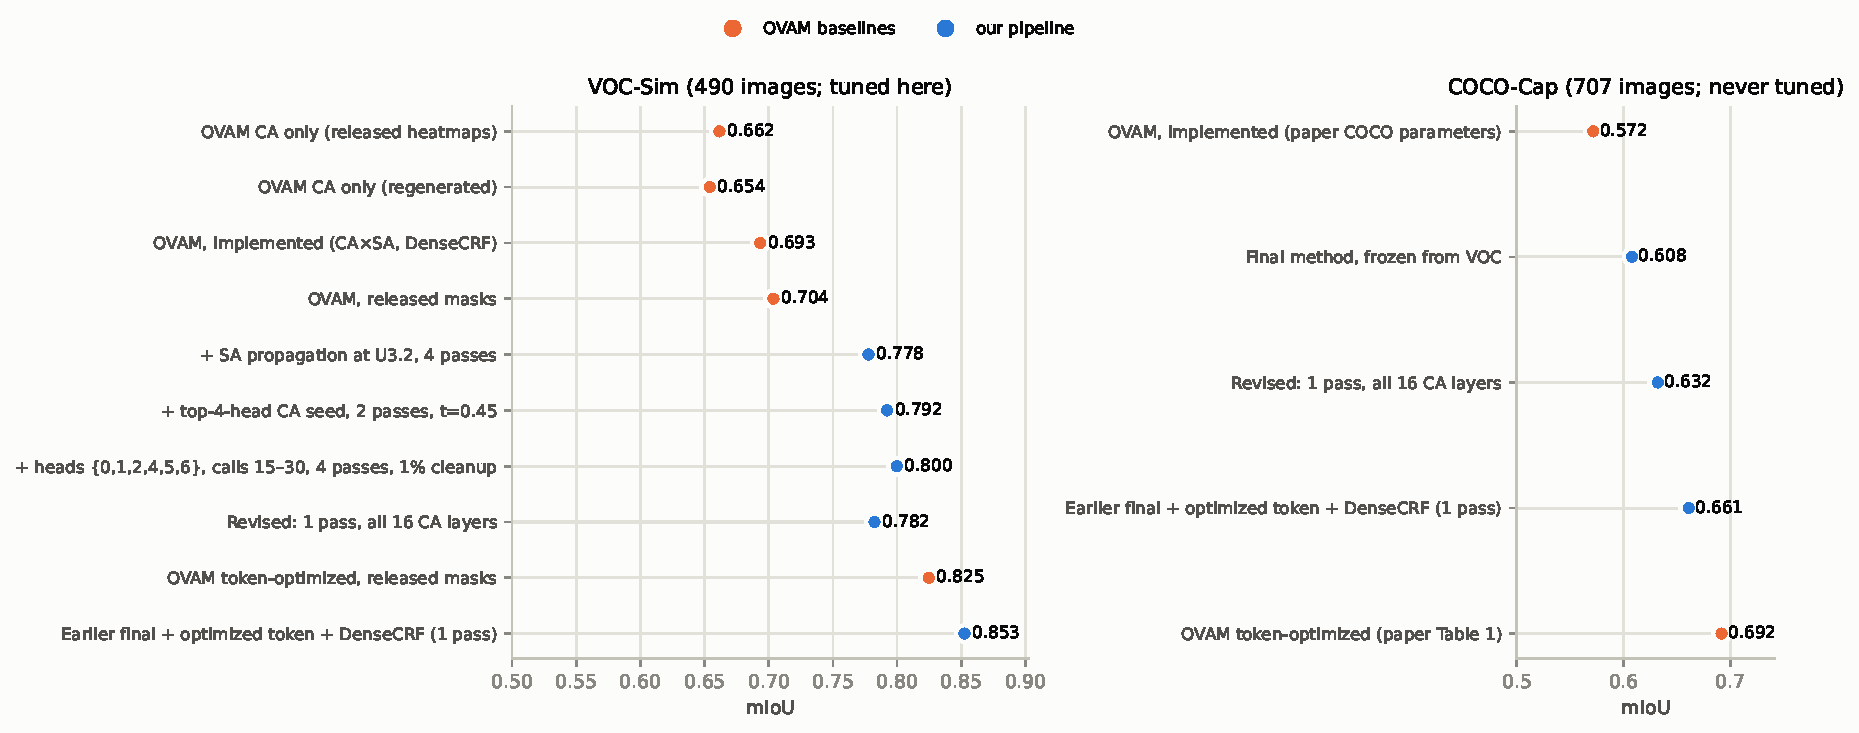
\includegraphics[width=1.0\linewidth]{evidence/figures/b_progression.pdf}
\caption{Each step of the method and the baselines. VOC-Sim values are in-sample; COCO-Cap was never used to choose the earlier final method.}\label{fig:b_progression}
\end{figure}
\begin{figure}[H]\centering
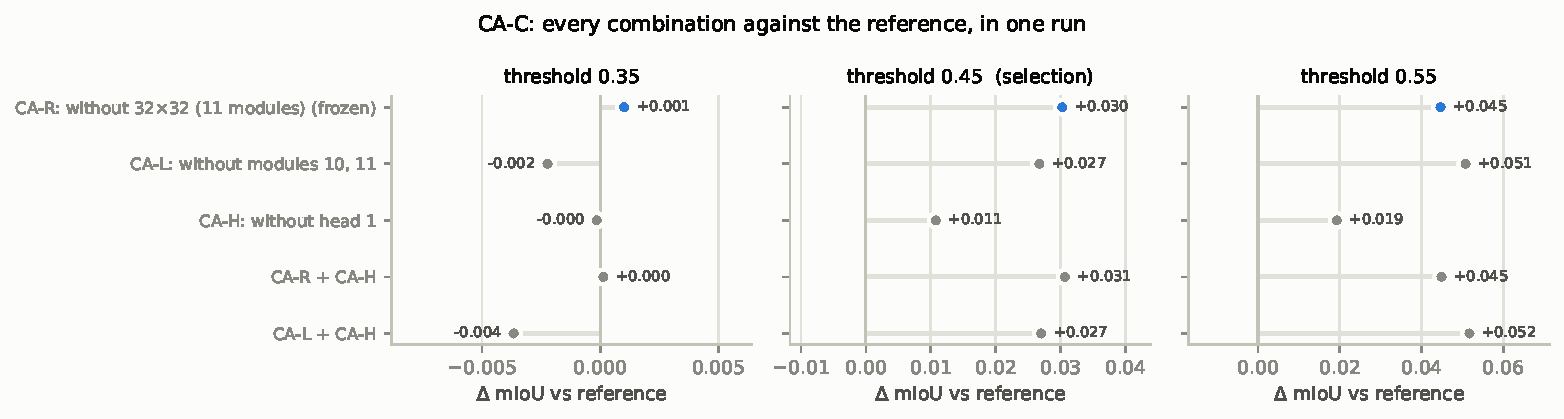
\includegraphics[width=1.0\linewidth]{evidence/figures/a3_ca_c_thresholds.pdf}
\caption{CA-C: change in mIoU of every combination against the reference at thresholds 0.35, 0.45 and 0.55 (blue = frozen).}\label{fig:a3_ca_c_thresholds}
\end{figure}
\begin{figure}[H]\centering
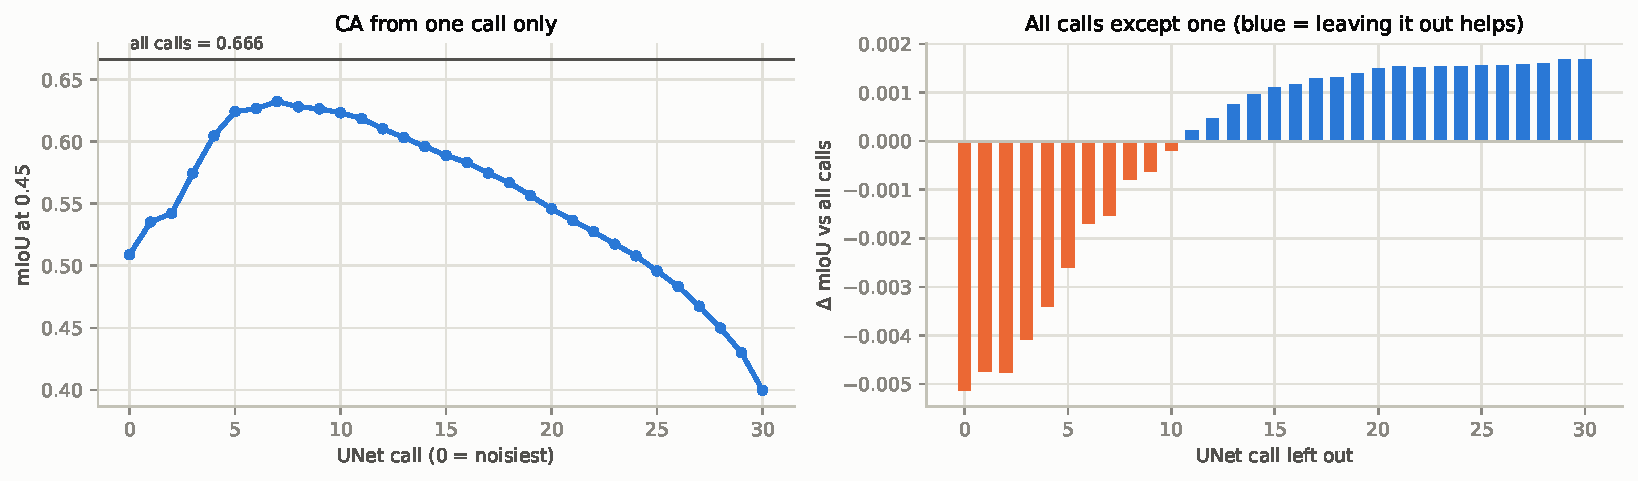
\includegraphics[width=1.0\linewidth]{evidence/figures/a2_ca_t_calls.pdf}
\caption{CA-T: CA from a single UNet call, and all calls except one.}\label{fig:a2_ca_t_calls}
\end{figure}
\begin{figure}[H]\centering
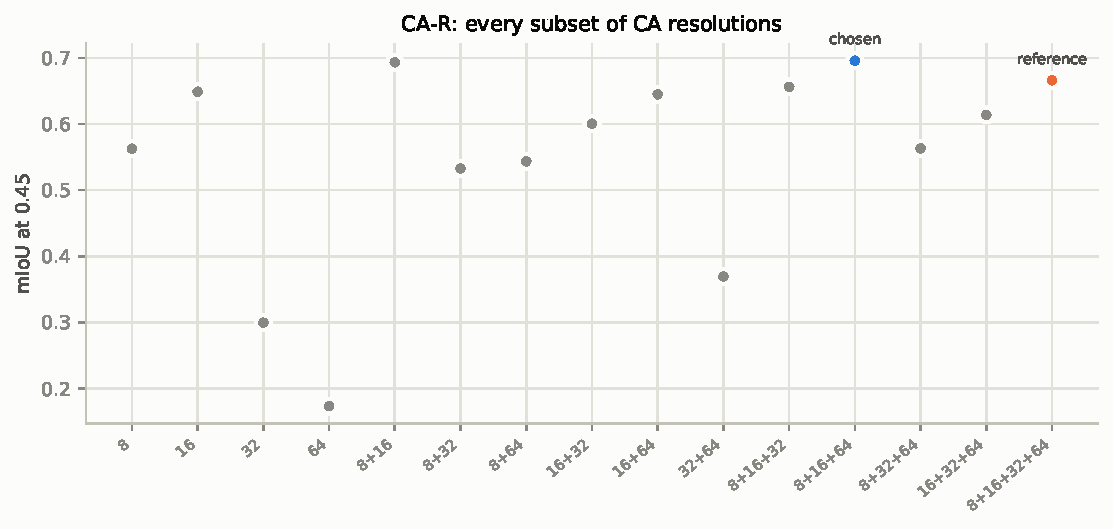
\includegraphics[width=0.75\linewidth]{evidence/figures/a2_ca_r_subsets.pdf}
\caption{CA-R: every subset of CA resolutions.}\label{fig:a2_ca_r_subsets}
\end{figure}
\begin{figure}[H]\centering
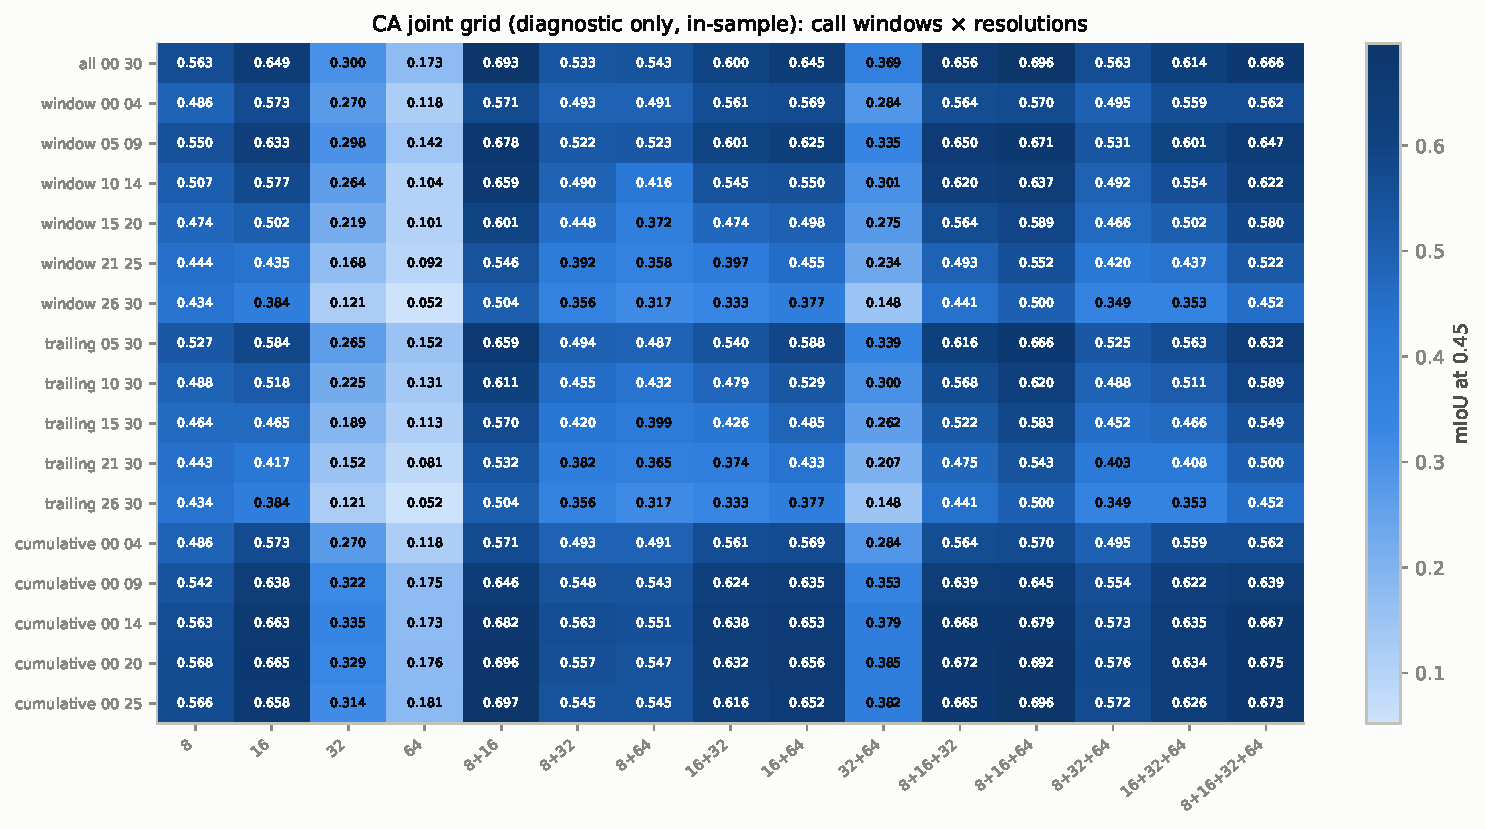
\includegraphics[width=0.95\linewidth]{evidence/figures/a2_joint_grid.pdf}
\caption{Joint grid of call windows and resolutions (diagnostic only).}\label{fig:a2_joint_grid}
\end{figure}
\begin{figure}[H]\centering
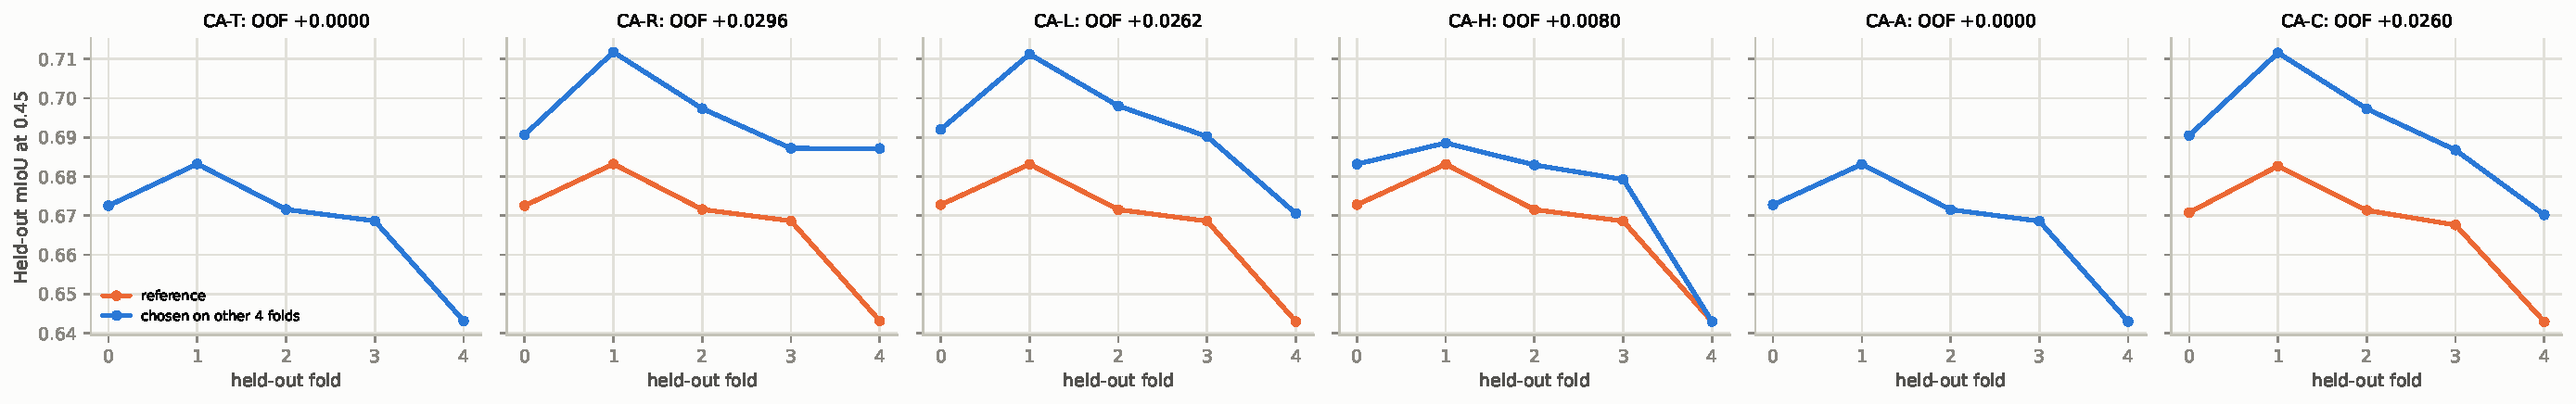
\includegraphics[width=1.0\linewidth]{evidence/figures/a_heldout_folds.pdf}
\caption{Controlled CA screens: held-out mIoU of the setting chosen on the other four folds, against the reference, per fold.}\label{fig:a_heldout_folds}
\end{figure}
\begin{figure}[H]\centering
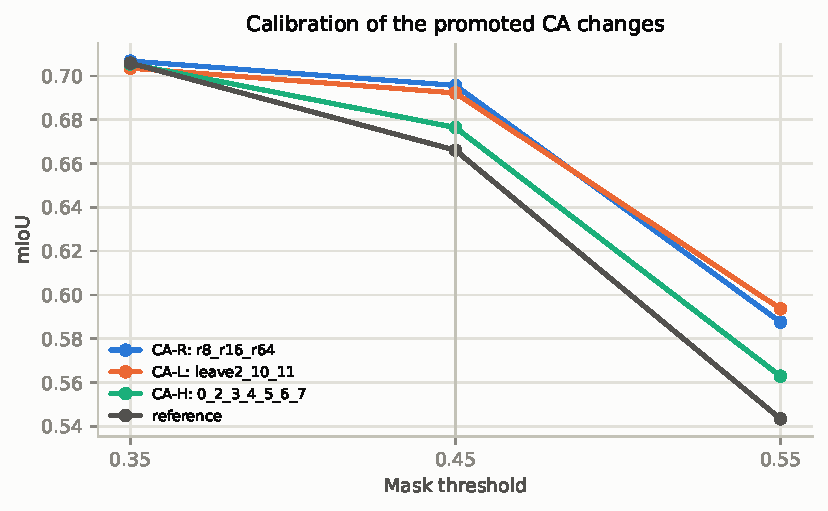
\includegraphics[width=0.6\linewidth]{evidence/figures/a_calibration.pdf}
\caption{Calibration of the promoted CA changes at thresholds 0.35, 0.45 and 0.55.}\label{fig:a_calibration}
\end{figure}
\begin{figure}[H]\centering
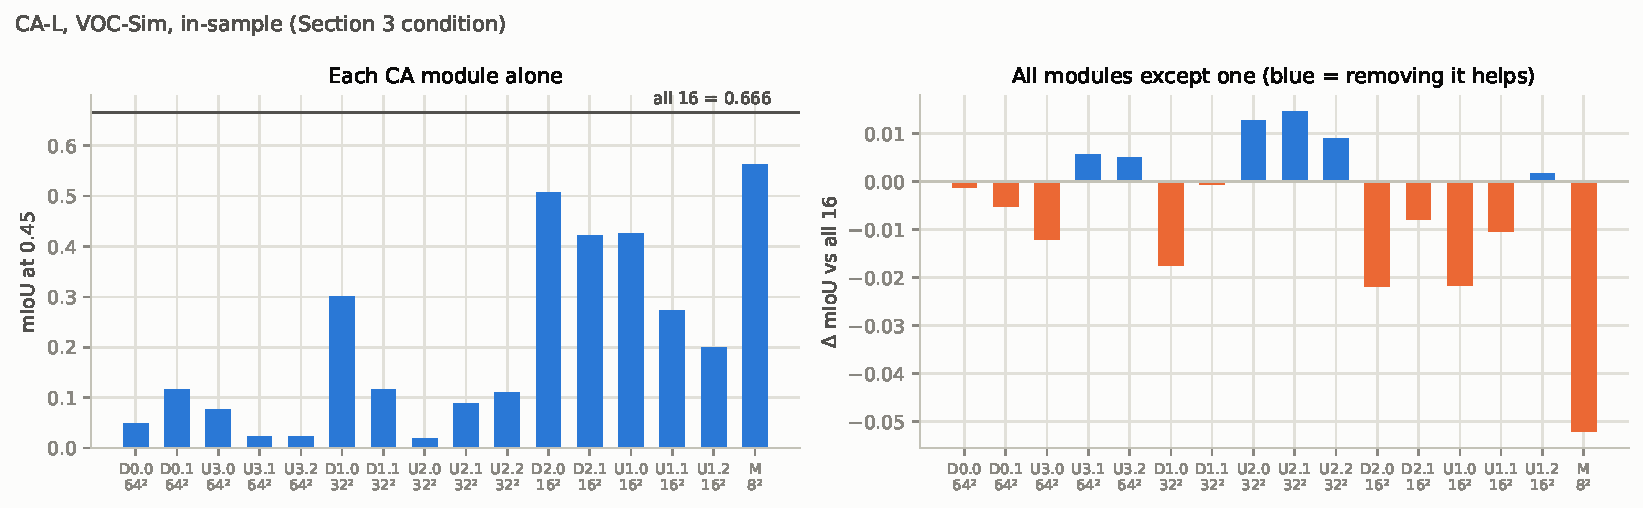
\includegraphics[width=1.0\linewidth]{evidence/figures/a1_ca_l_single_leave1.pdf}
\caption{CA-L: each CA module alone (left) and all modules except one (right).}\label{fig:a1_ca_l_single_leave1}
\end{figure}
\begin{figure}[H]\centering
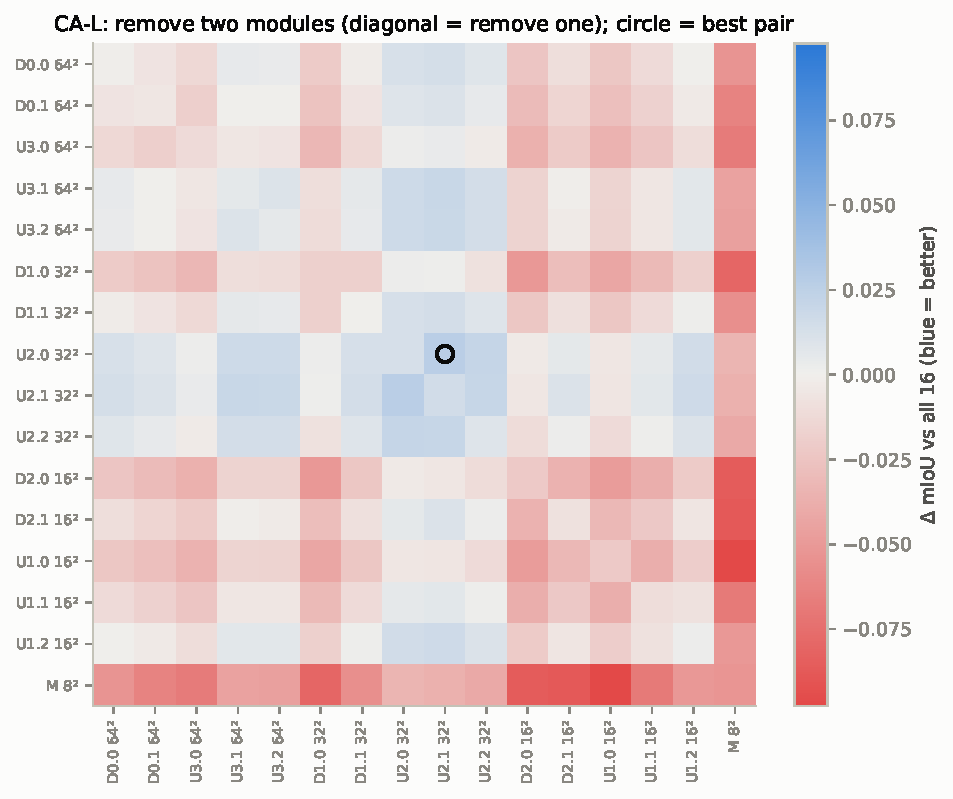
\includegraphics[width=0.7\linewidth]{evidence/figures/a1_ca_l_leave2_heatmap.pdf}
\caption{CA-L: all 120 leave-two-out configurations; the diagonal is leave-one-out.}\label{fig:a1_ca_l_leave2_heatmap}
\end{figure}
\begin{figure}[H]\centering
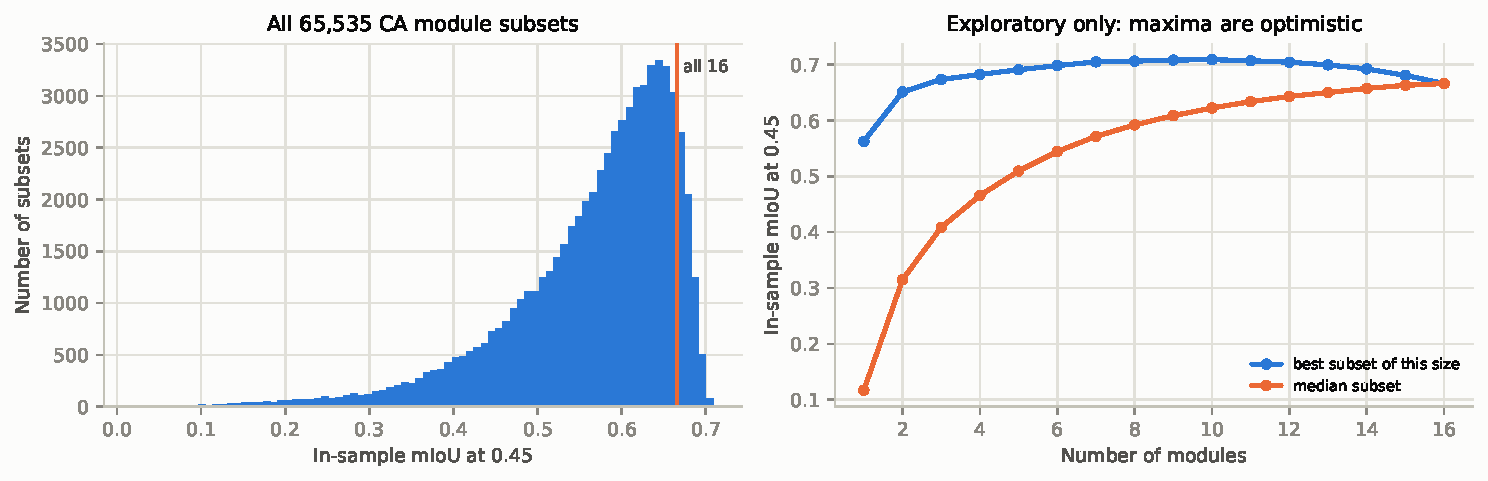
\includegraphics[width=1.0\linewidth]{evidence/figures/a1_exhaustive.pdf}
\caption{All 65,535 CA module subsets (exploratory; the maximum is not eligible for selection).}\label{fig:a1_exhaustive}
\end{figure}
\begin{figure}[H]\centering
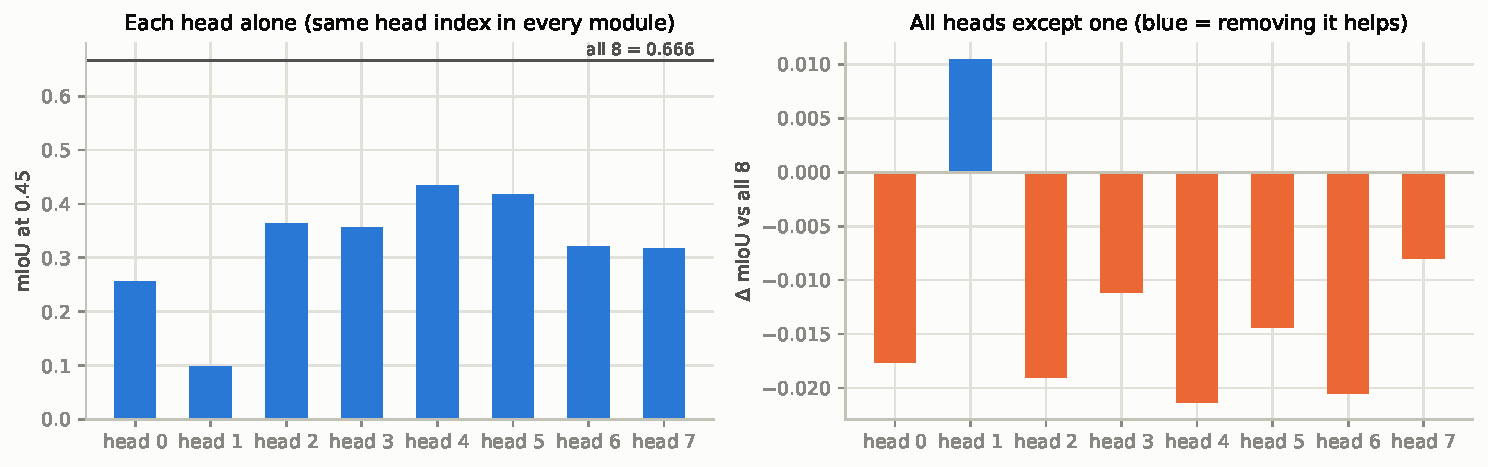
\includegraphics[width=1.0\linewidth]{evidence/figures/a1_ca_h_single_leave1.pdf}
\caption{CA-H: each head alone and all heads except one (the same head index in every module).}\label{fig:a1_ca_h_single_leave1}
\end{figure}
\begin{figure}[H]\centering
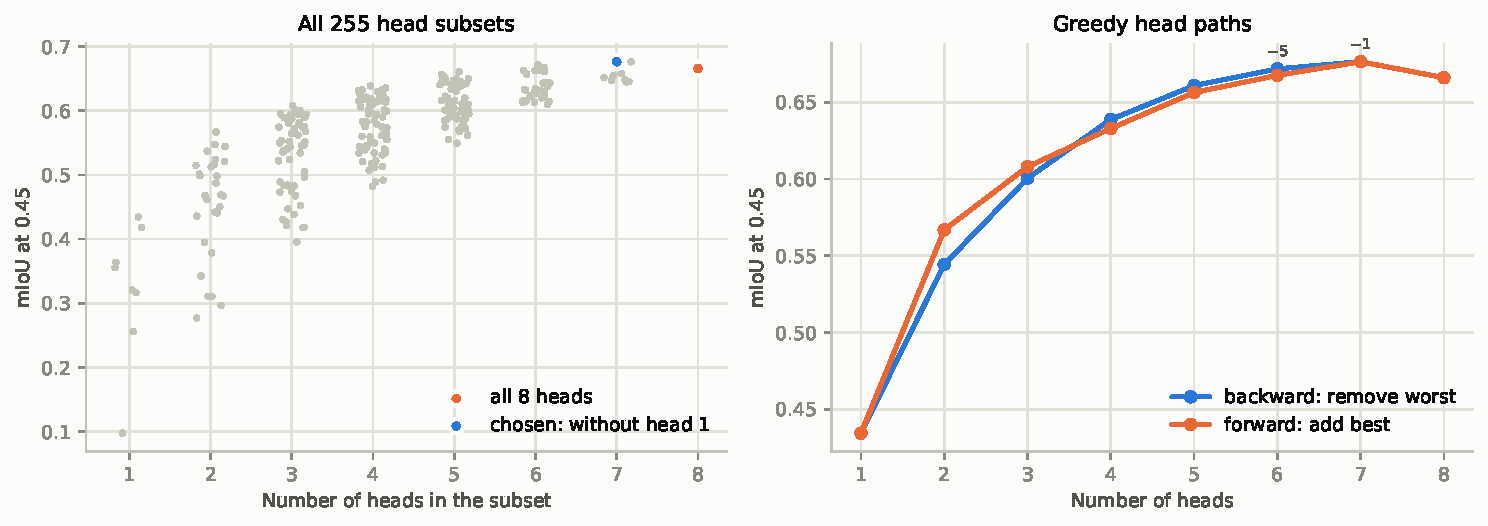
\includegraphics[width=1.0\linewidth]{evidence/figures/a1_ca_h_subsets_greedy.pdf}
\caption{CA-H: all 255 head subsets by size, and the greedy removal and addition paths.}\label{fig:a1_ca_h_subsets_greedy}
\end{figure}
\begin{figure}[H]\centering
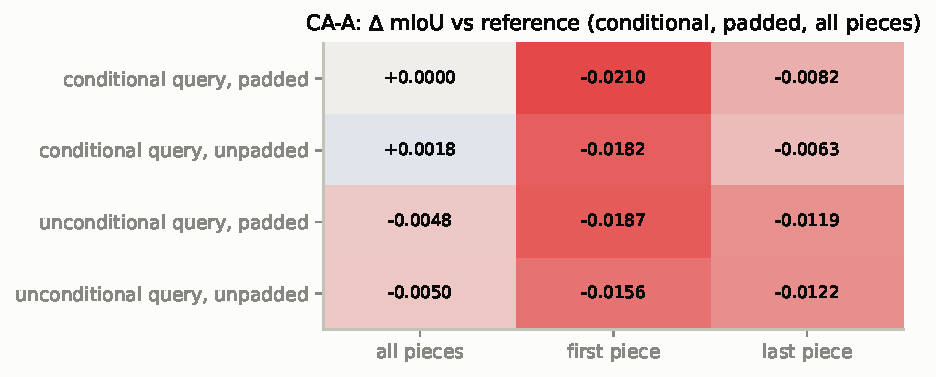
\includegraphics[width=0.65\linewidth]{evidence/figures/a1_ca_a_grid.pdf}
\caption{CA-A: change in mIoU of each attribution convention against the reference.}\label{fig:a1_ca_a_grid}
\end{figure}
\begin{figure}[H]\centering
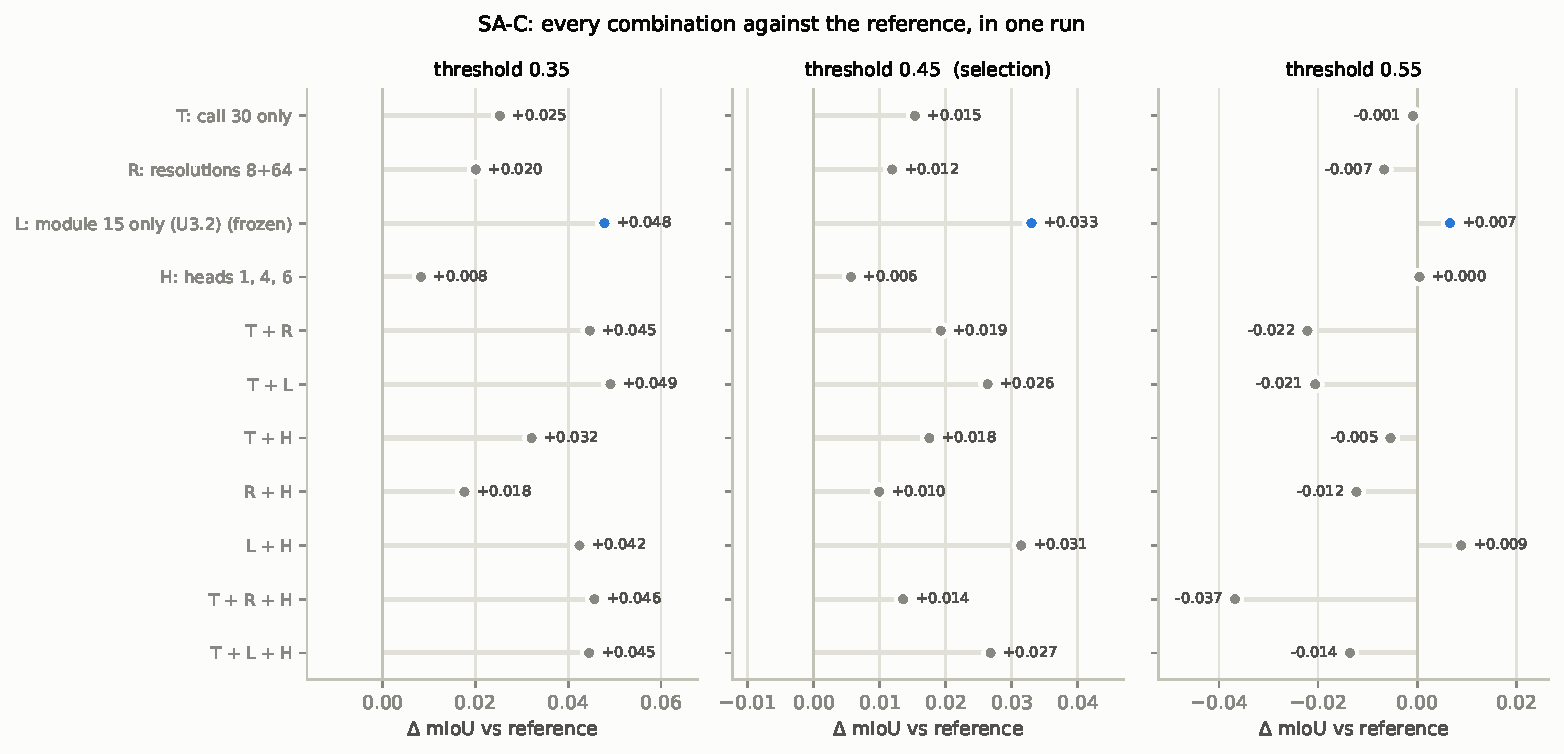
\includegraphics[width=1.0\linewidth]{evidence/figures/a6_sa_c_thresholds.pdf}
\caption{SA-C: change in mIoU of every combination against the SA reference at thresholds 0.35, 0.45 and 0.55 (blue = frozen).}\label{fig:a6_sa_c_thresholds}
\end{figure}
\begin{figure}[H]\centering
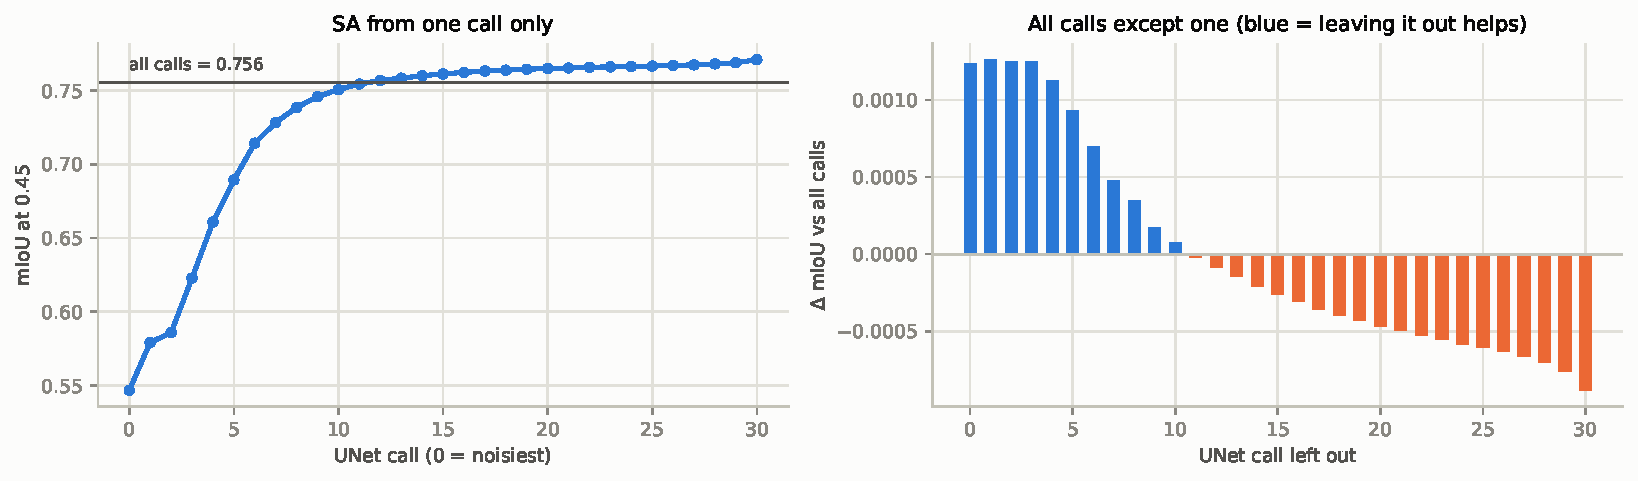
\includegraphics[width=1.0\linewidth]{evidence/figures/a5_sa_t_calls.pdf}
\caption{SA-T: SA from a single UNet call, and all calls except one.}\label{fig:a5_sa_t_calls}
\end{figure}
\begin{figure}[H]\centering
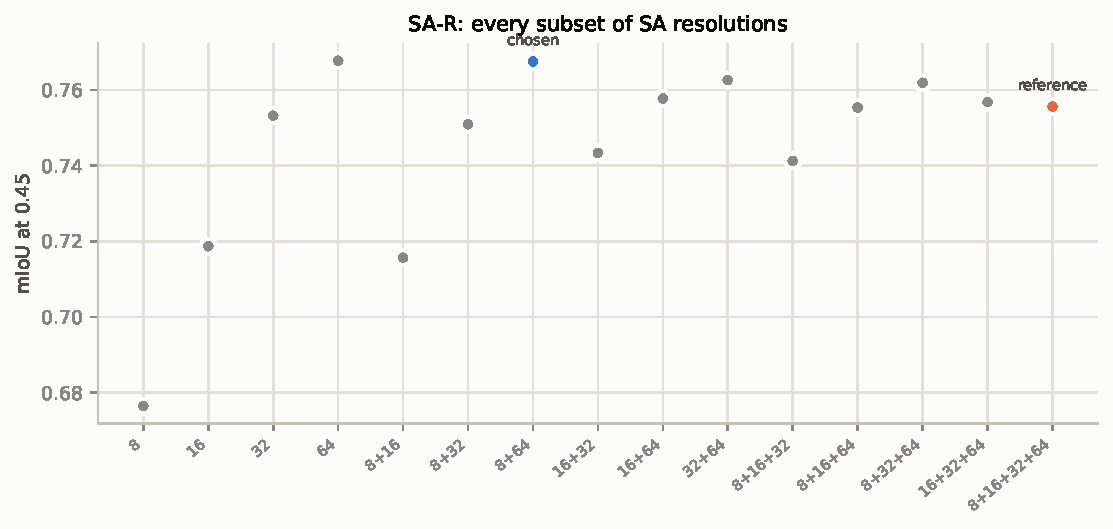
\includegraphics[width=0.75\linewidth]{evidence/figures/a5_sa_r_subsets.pdf}
\caption{SA-R: every subset of SA resolutions.}\label{fig:a5_sa_r_subsets}
\end{figure}
\begin{figure}[H]\centering
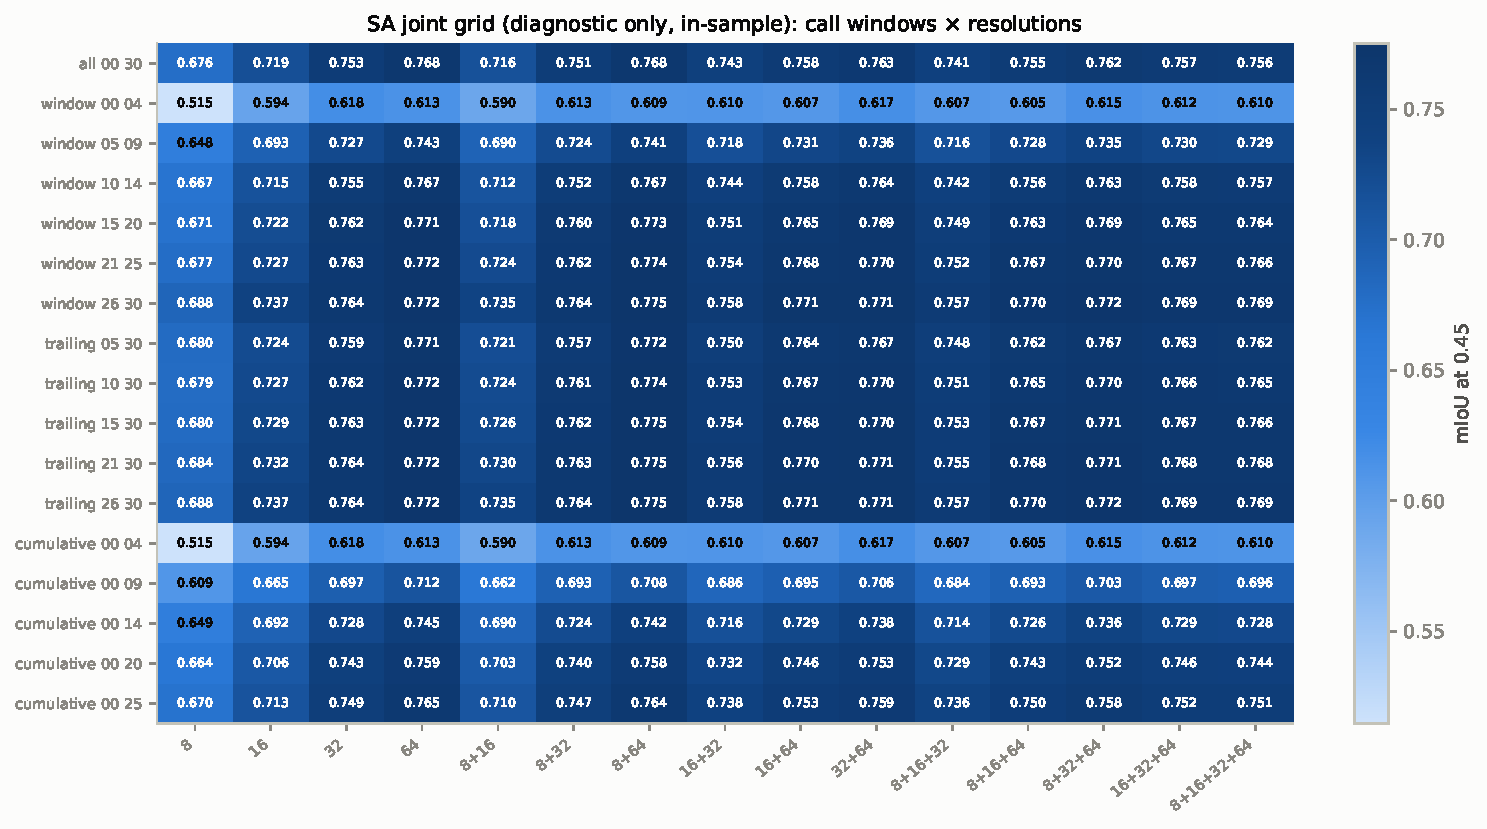
\includegraphics[width=0.95\linewidth]{evidence/figures/a5_joint_grid.pdf}
\caption{SA joint grid of call windows and resolutions (diagnostic only).}\label{fig:a5_joint_grid}
\end{figure}
\begin{figure}[H]\centering
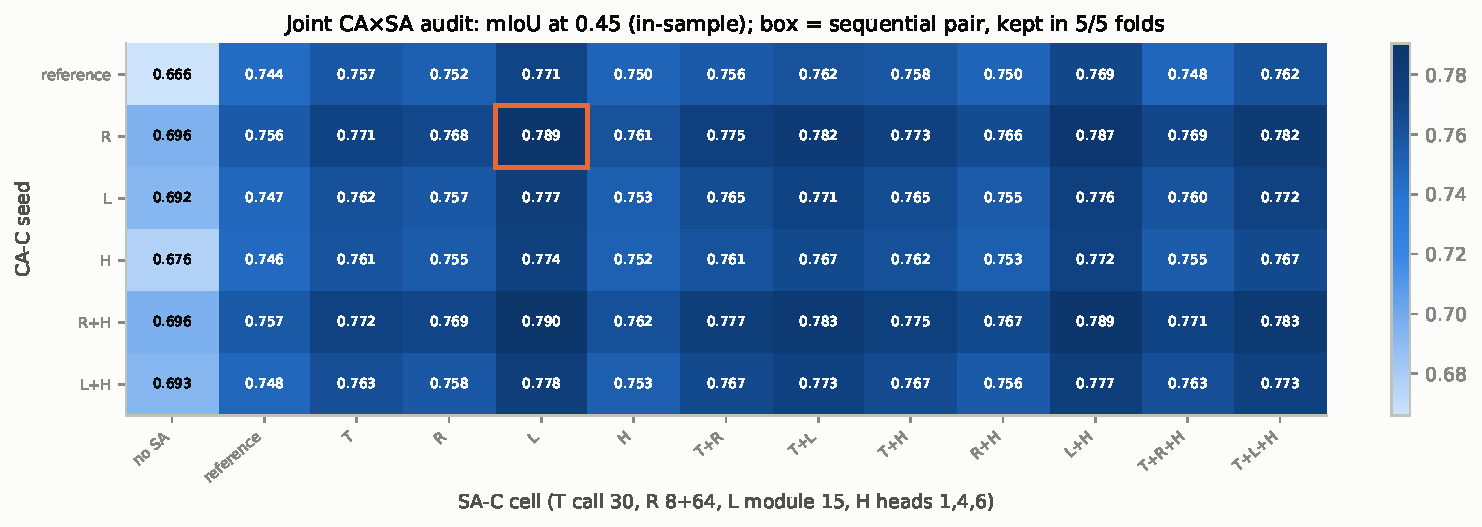
\includegraphics[width=1.0\linewidth]{evidence/figures/a7_joint_audit.pdf}
\caption{Joint CA$\times$SA audit: mIoU of all 78 cells (in-sample); the box is the frozen pair.}\label{fig:a7_joint_audit}
\end{figure}
\begin{figure}[H]\centering
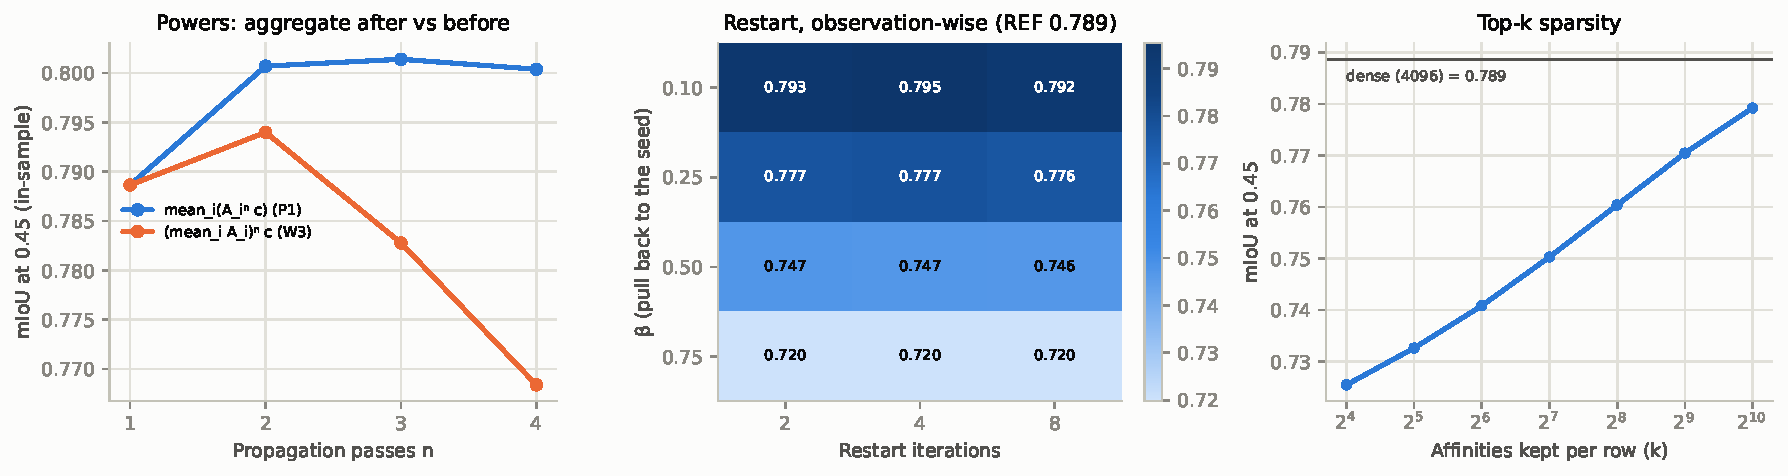
\includegraphics[width=1.0\linewidth]{evidence/figures/a8_propagation.pdf}
\caption{Propagation: passes under both aggregation orders, restart, and top-k sparsity (in-sample).}\label{fig:a8_propagation}
\end{figure}
\begin{figure}[H]\centering
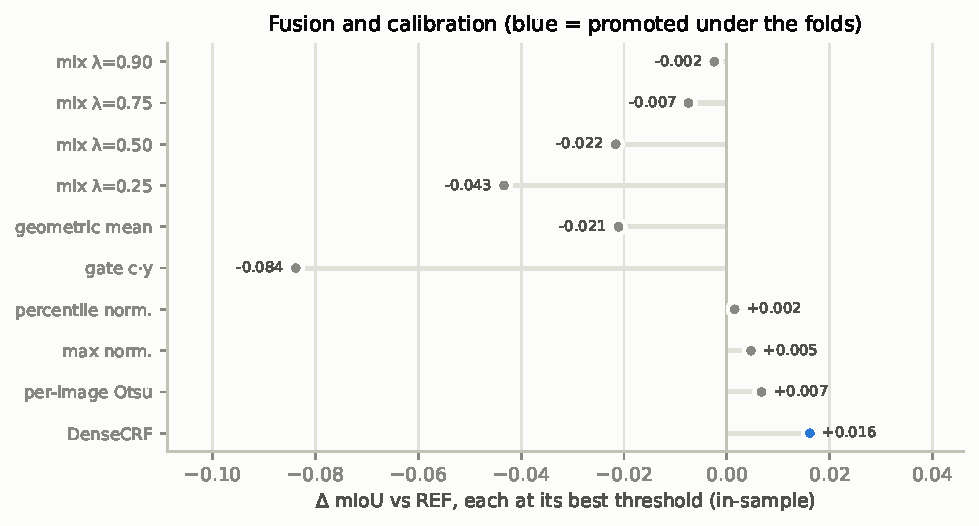
\includegraphics[width=0.7\linewidth]{evidence/figures/a9_fusion.pdf}
\caption{Fusion and calibration: change against REF, each at its best threshold (in-sample).}\label{fig:a9_fusion}
\end{figure}
\begin{figure}[H]\centering
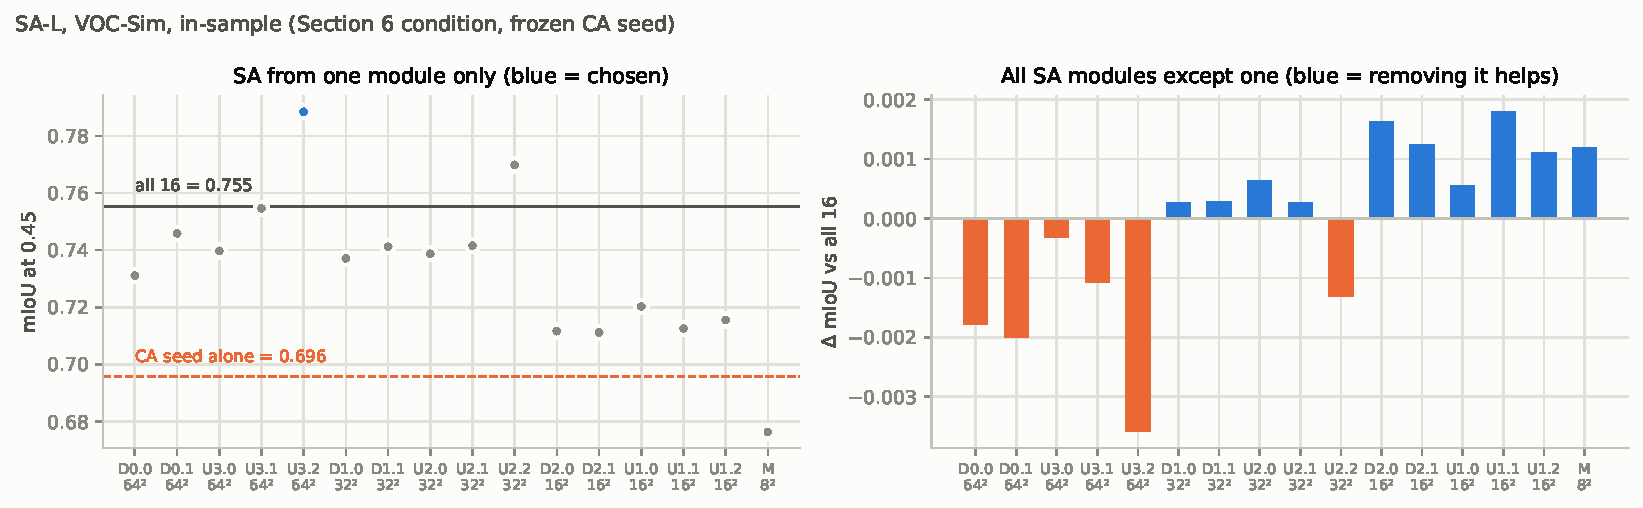
\includegraphics[width=1.0\linewidth]{evidence/figures/a4_sa_l_single_leave1.pdf}
\caption{SA-L: SA from one module only, and all SA modules except one (frozen CA seed).}\label{fig:a4_sa_l_single_leave1}
\end{figure}
\begin{figure}[H]\centering
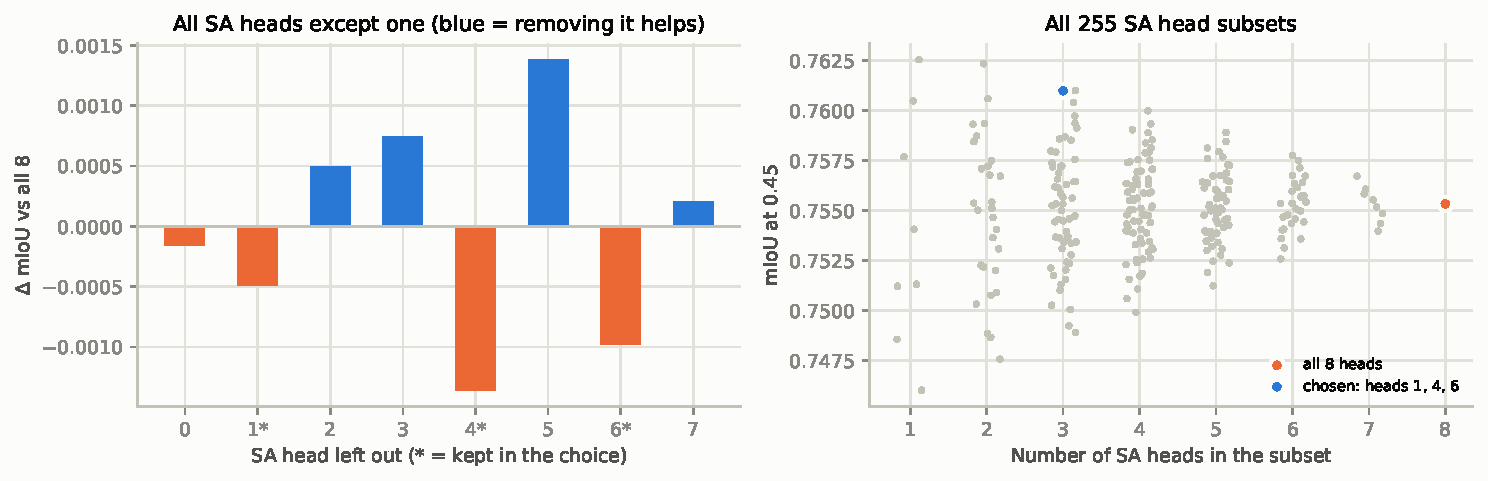
\includegraphics[width=1.0\linewidth]{evidence/figures/a4_sa_h.pdf}
\caption{SA-H: leaving out one SA head, and all 255 SA head subsets by size.}\label{fig:a4_sa_h}
\end{figure}
\begin{figure}[H]\centering
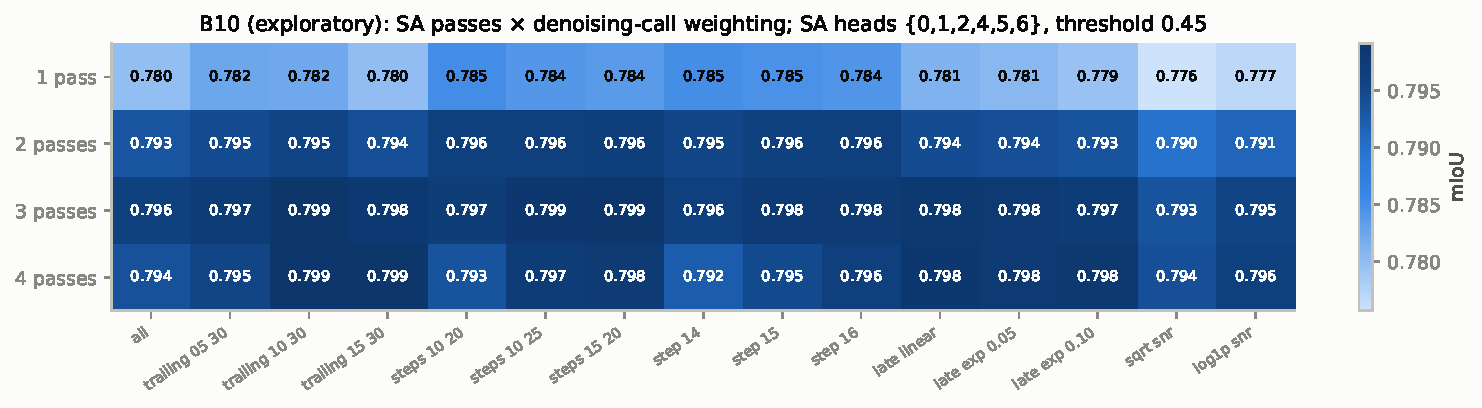
\includegraphics[width=1.0\linewidth]{evidence/figures/b_joint_passes_time.pdf}
\caption{Exploratory B10: SA passes by denoising-call weighting (in-sample).}\label{fig:b_joint_passes_time}
\end{figure}
\begin{figure}[H]\centering
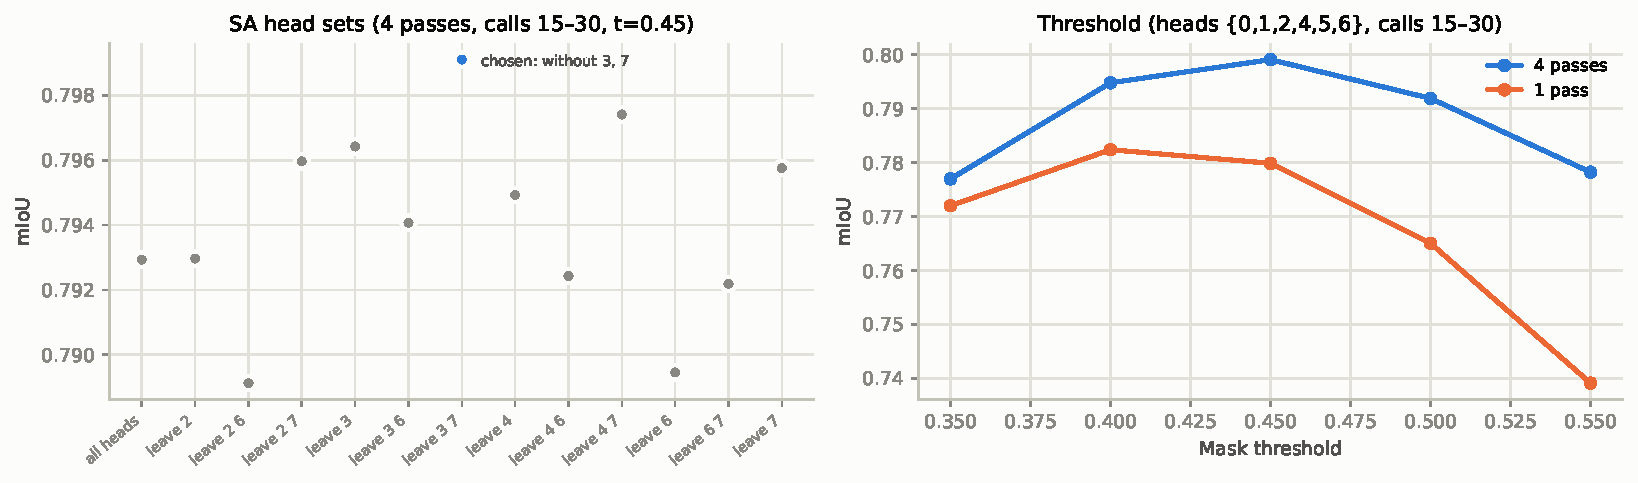
\includegraphics[width=1.0\linewidth]{evidence/figures/b_joint_heads_threshold.pdf}
\caption{Exploratory B10: SA head subsets and the mask threshold (in-sample).}\label{fig:b_joint_heads_threshold}
\end{figure}
\begin{figure}[H]\centering
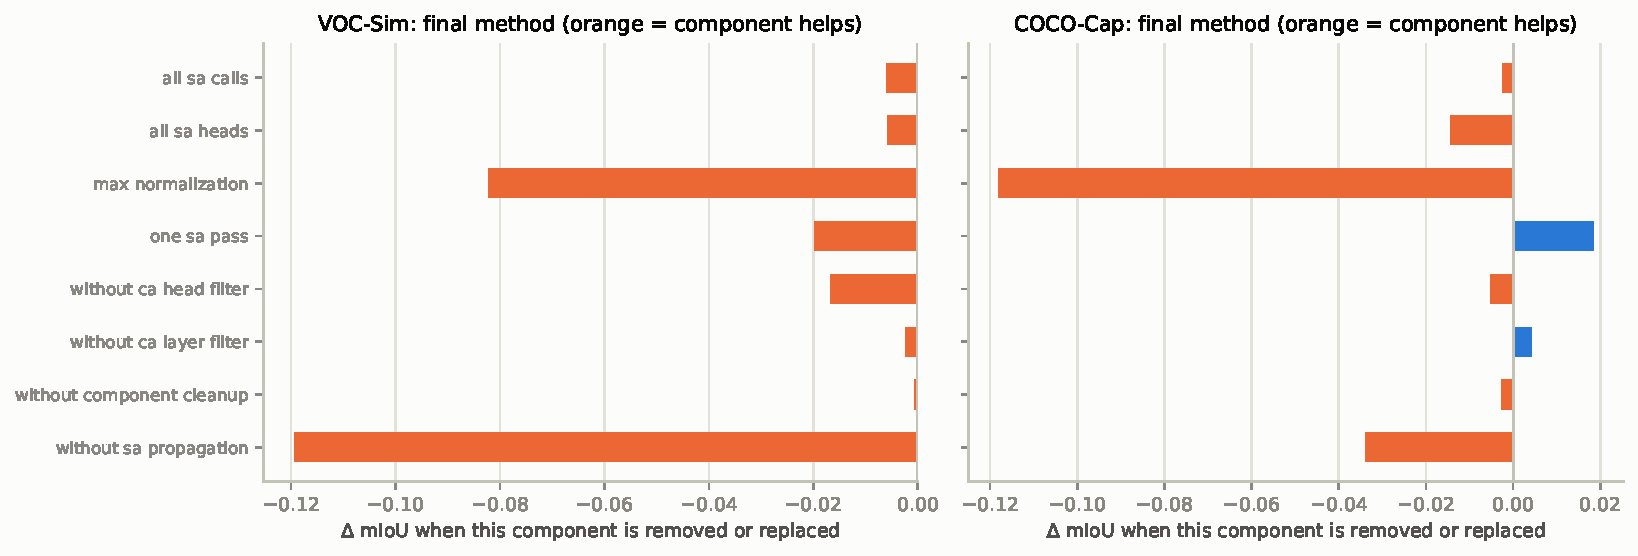
\includegraphics[width=1.0\linewidth]{evidence/figures/b_component_ablation.pdf}
\caption{Removing one component of the earlier final method, on VOC-Sim and on the untuned COCO-Cap.}\label{fig:b_component_ablation}
\end{figure}
\begin{figure}[H]\centering
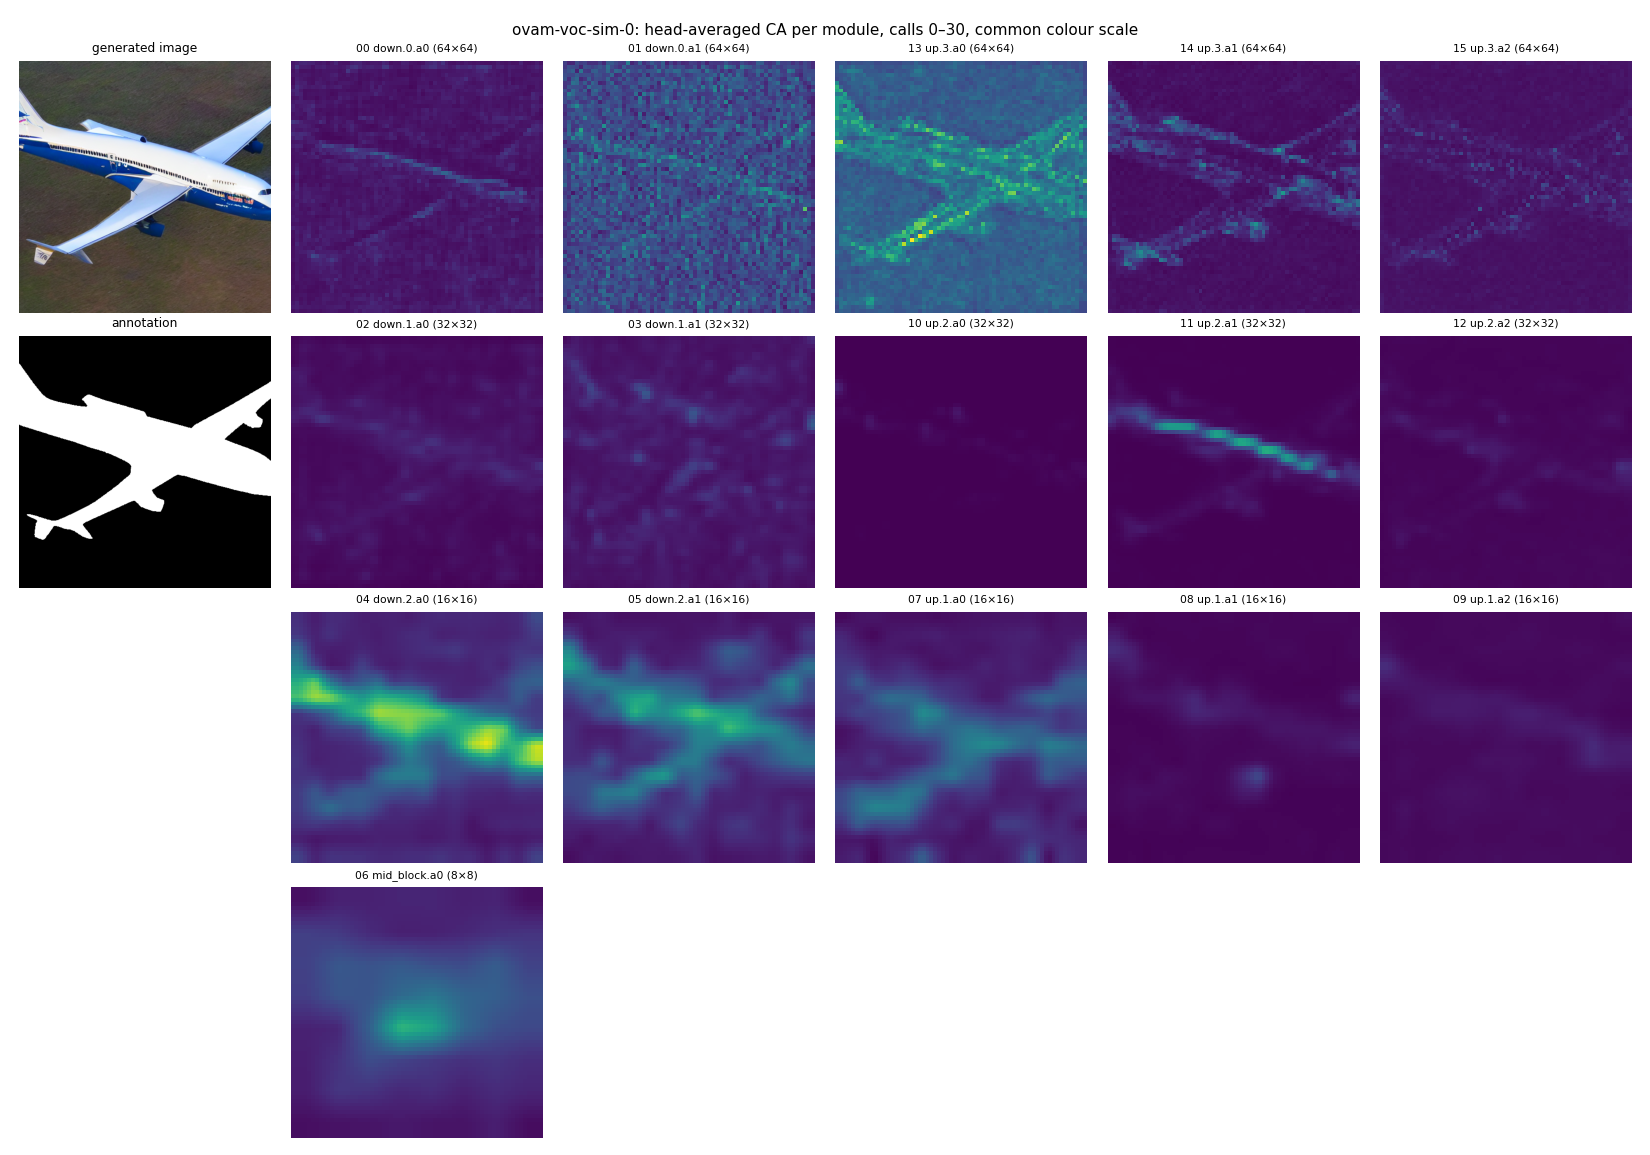
\includegraphics[width=0.85\linewidth]{evidence/figures/ovam-voc-sim-0_ca_modules.png}
\caption{Head-averaged cross-attention of every module for ovam-voc-sim-0, calls 0--30, common colour scale, one row per resolution.}
\end{figure}
\begin{figure}[H]\centering
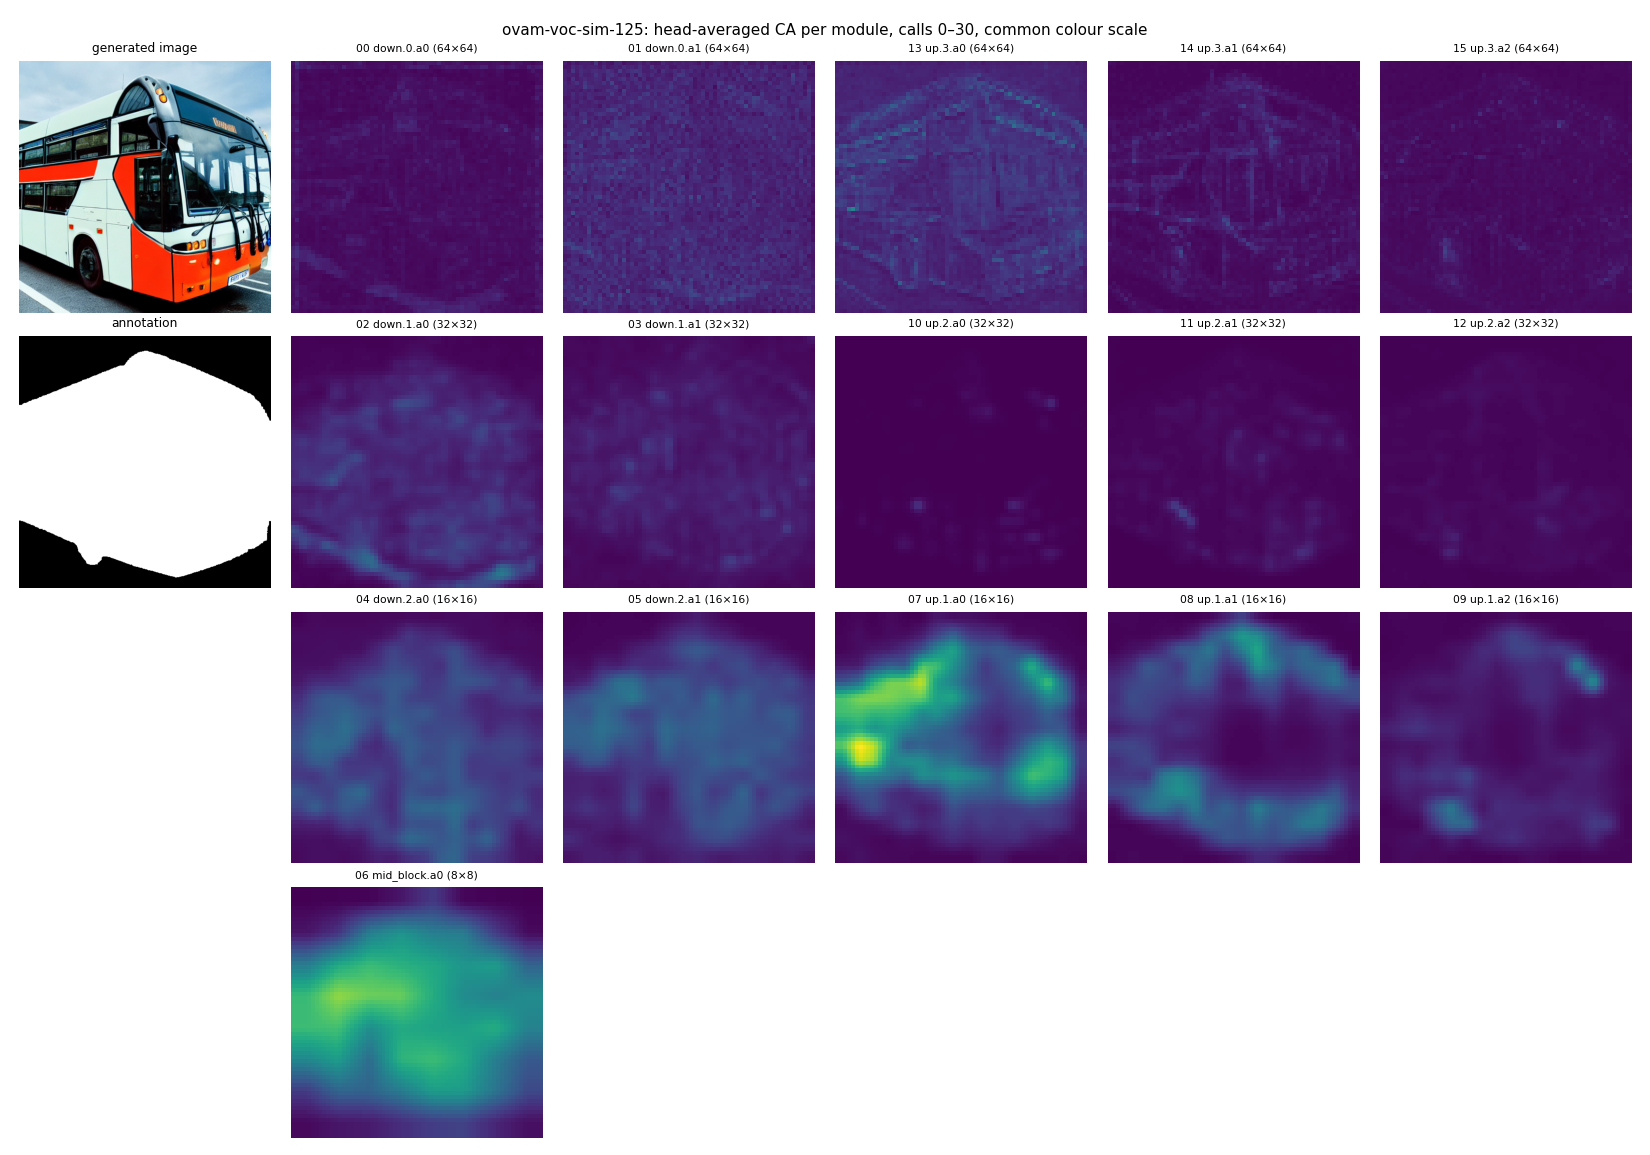
\includegraphics[width=0.85\linewidth]{evidence/figures/ovam-voc-sim-125_ca_modules.png}
\caption{Head-averaged cross-attention of every module for ovam-voc-sim-125, calls 0--30, common colour scale, one row per resolution.}
\end{figure}
\begin{figure}[H]\centering
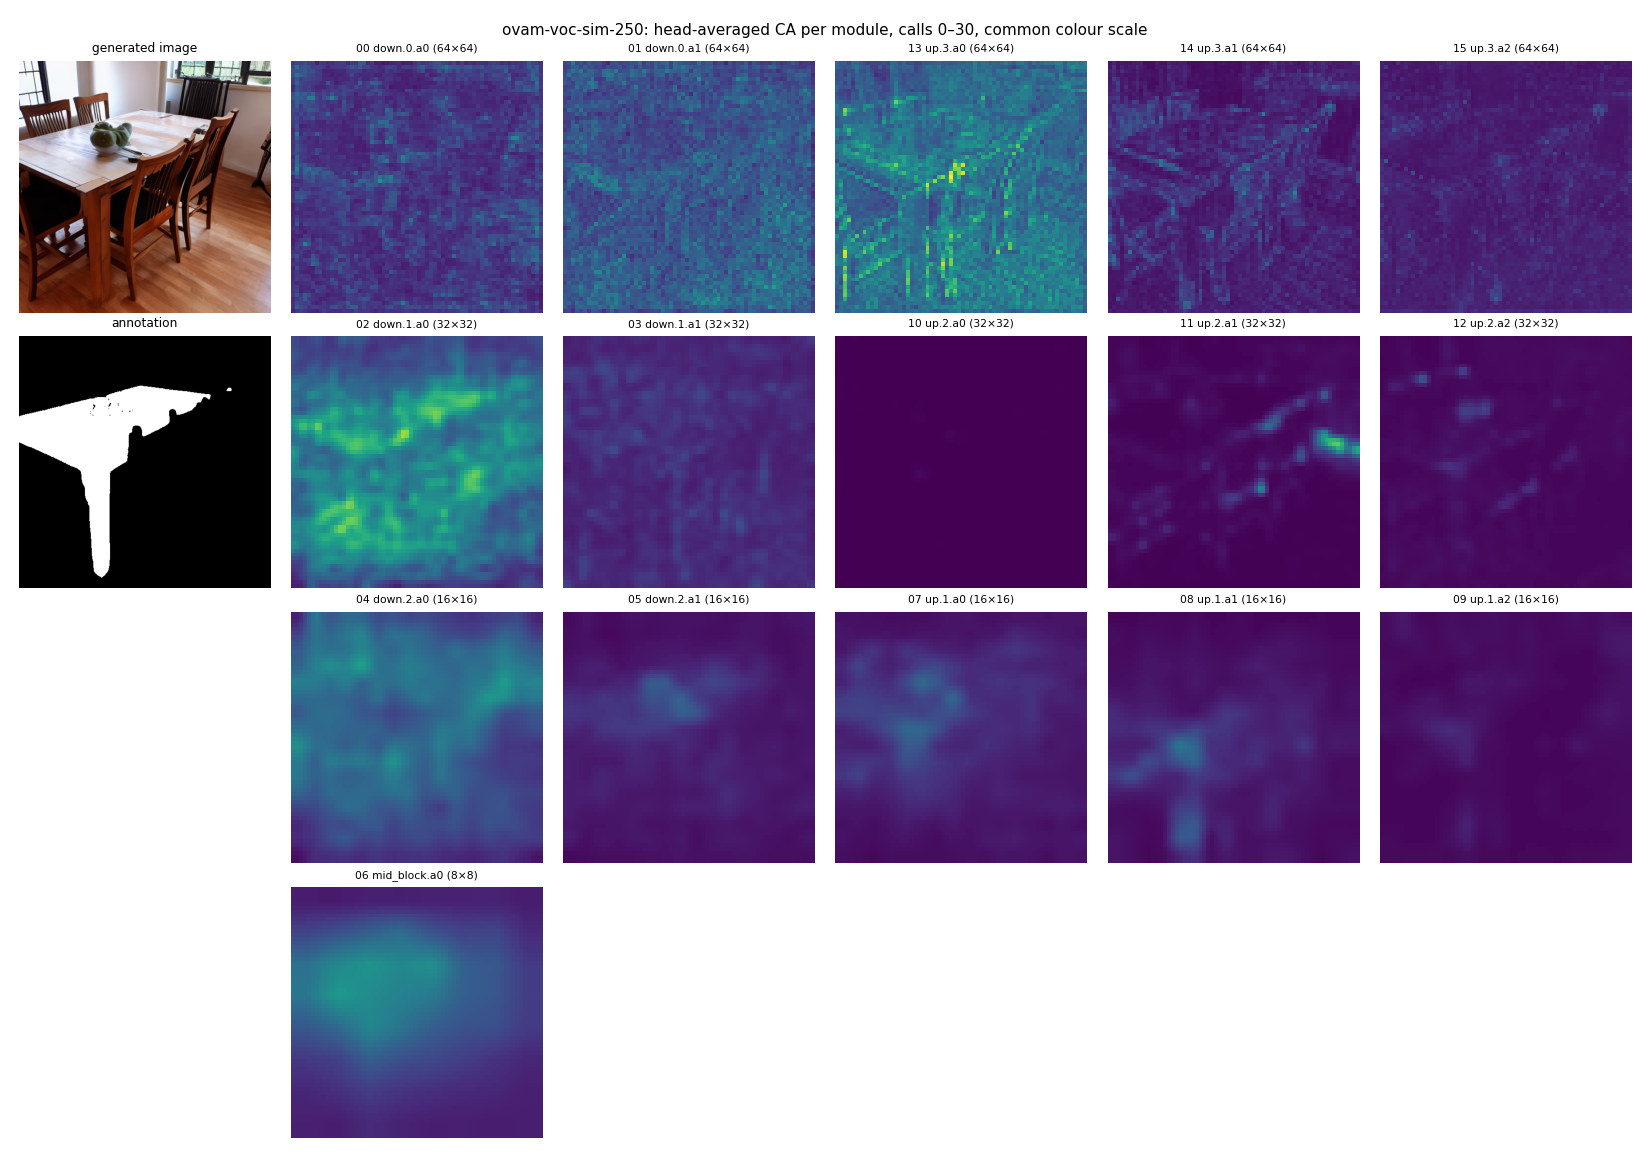
\includegraphics[width=0.85\linewidth]{evidence/figures/ovam-voc-sim-250_ca_modules.png}
\caption{Head-averaged cross-attention of every module for ovam-voc-sim-250, calls 0--30, common colour scale, one row per resolution.}
\end{figure}
\begin{figure}[H]\centering
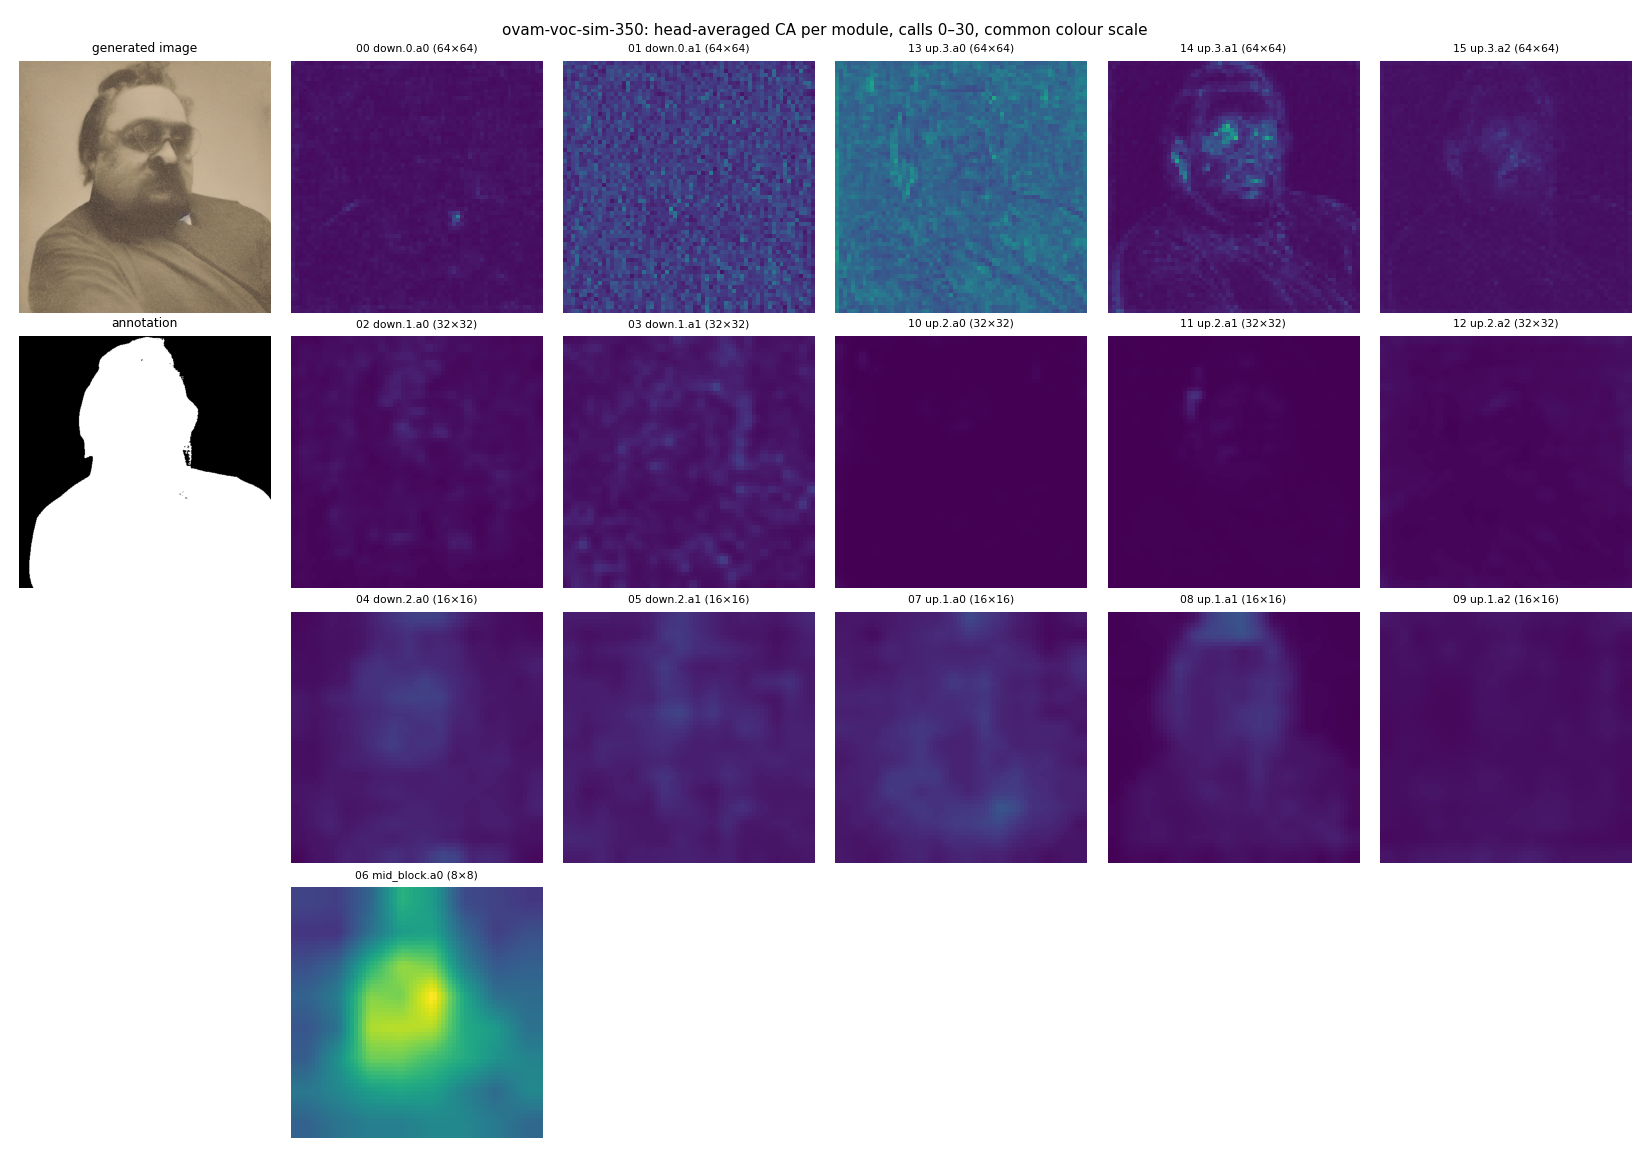
\includegraphics[width=0.85\linewidth]{evidence/figures/ovam-voc-sim-350_ca_modules.png}
\caption{Head-averaged cross-attention of every module for ovam-voc-sim-350, calls 0--30, common colour scale, one row per resolution.}
\end{figure}
\begin{table}[H]\centering\scriptsize\setlength{\tabcolsep}{3pt}
\begin{tabular}{>{\raggedright\arraybackslash}p{1.92cm}>{\raggedright\arraybackslash}p{7.65cm}r>{\raggedright\arraybackslash}p{3.85cm}}
\toprule
Dataset & Method & mIoU & Evidence \\
\midrule
VOC-Sim & OVAM CA only (released heatmaps) & 0.6616 & B16 \\
VOC-Sim & OVAM CA only (regenerated) & 0.6540 & B8 \\
VOC-Sim & OVAM, implemented (CA$\times$SA, DenseCRF) & 0.6934 & attention\_\allowbreak{}analysis.md \\
VOC-Sim & OVAM, released masks & 0.7036 & B16 \\
VOC-Sim & + SA propagation at U3.2, 4 passes & 0.7777 & B8 \\
VOC-Sim & + top-4-head CA seed, 2 passes, t=0.45 & 0.7922 & B9 \\
VOC-Sim & + heads \{0,1,2,4,5,6\}, calls 15--30, 4 passes, 1\% cleanup & 0.7997 & B10 \\
VOC-Sim & Revised: 1 pass, all 16 CA layers & 0.7824 & B13 \\
VOC-Sim & OVAM token-optimized, released masks & 0.8247 & B16 \\
VOC-Sim & Earlier final + optimized token + DenseCRF (1 pass) & 0.8525 & B17 \\
COCO-Cap & OVAM, implemented (paper COCO parameters) & 0.5717 & B17 \\
COCO-Cap & Final method, frozen from VOC & 0.6080 & B12 \\
COCO-Cap & Revised: 1 pass, all 16 CA layers & 0.6322 & B13 \\
COCO-Cap & Earlier final + optimized token + DenseCRF (1 pass) & 0.6612 & B17 \\
COCO-Cap & OVAM token-optimized (paper Table 1) & 0.6920 & OVAM paper \\
\bottomrule
\end{tabular}
\caption{How the method developed, with the baselines it is compared against}\label{tab:b_progression}
\end{table}

\begin{table}[H]\centering\scriptsize\setlength{\tabcolsep}{3pt}
\begin{tabular}{>{\raggedright\arraybackslash}p{1.92cm}>{\raggedright\arraybackslash}p{7.05cm}r}
\toprule
Dataset & Configuration & mIoU \\
\midrule
VOC-Sim & ovam\_\allowbreak{}implemented & 0.6945 \\
VOC-Sim & plain\_\allowbreak{}top4/\allowbreak{}sa\_\allowbreak{}iter1 & 0.7802 \\
VOC-Sim & plain\_\allowbreak{}top4/\allowbreak{}sa\_\allowbreak{}iter1+crf & 0.7957 \\
VOC-Sim & opt\_\allowbreak{}top4/\allowbreak{}sa\_\allowbreak{}iter1 & 0.8347 \\
VOC-Sim & opt\_\allowbreak{}top4/\allowbreak{}sa\_\allowbreak{}iter1+crf & 0.8525 \\
VOC-Sim & opt\_\allowbreak{}all16/\allowbreak{}sa\_\allowbreak{}iter1+crf & 0.8553 \\
VOC-Sim & plain\_\allowbreak{}top4/\allowbreak{}sa\_\allowbreak{}iter4 & 0.8000 \\
VOC-Sim & opt\_\allowbreak{}top4/\allowbreak{}sa\_\allowbreak{}iter4+crf & 0.8521 \\
COCO-Cap & ovam\_\allowbreak{}implemented & 0.5717 \\
COCO-Cap & plain\_\allowbreak{}top4/\allowbreak{}sa\_\allowbreak{}iter1 & 0.6264 \\
COCO-Cap & plain\_\allowbreak{}top4/\allowbreak{}sa\_\allowbreak{}iter1+crf & 0.6432 \\
COCO-Cap & opt\_\allowbreak{}top4/\allowbreak{}sa\_\allowbreak{}iter1 & 0.6419 \\
COCO-Cap & opt\_\allowbreak{}top4/\allowbreak{}sa\_\allowbreak{}iter1+crf & 0.6612 \\
COCO-Cap & opt\_\allowbreak{}all16/\allowbreak{}sa\_\allowbreak{}iter1+crf & 0.6552 \\
COCO-Cap & plain\_\allowbreak{}top4/\allowbreak{}sa\_\allowbreak{}iter4 & 0.6077 \\
COCO-Cap & opt\_\allowbreak{}top4/\allowbreak{}sa\_\allowbreak{}iter4+crf & 0.6369 \\
VOC-Sim & released OVAM token-optimized masks & 0.8247 \\
COCO-Cap & OVAM token-optimized (paper) & 0.6920 \\
\bottomrule
\end{tabular}
\caption{OVAM optimized token and DenseCRF on the earlier final method (exploratory)}\label{tab:b_token_crf}
\end{table}

{\scriptsize\setlength{\tabcolsep}{3pt}
\begin{longtable}{>{\raggedright\arraybackslash}p{4.94cm}>{\raggedright\arraybackslash}p{1.92cm}>{\raggedright\arraybackslash}p{4.68cm}rr}
\caption{Remove-one-component ablations of the final and revised systems}\label{tab:b_component_ablations}\\
\toprule
System & Dataset & Change & mIoU & $\Delta$ vs full \\
\midrule
\endfirsthead
\toprule
System & Dataset & Change & mIoU & $\Delta$ vs full \\
\midrule
\endhead
final (4 passes, 12 layers) & VOC-Sim & all sa calls & 0.7938 & -0.0060 \\
final (4 passes, 12 layers) & VOC-Sim & all sa heads & 0.7940 & -0.0059 \\
final (4 passes, 12 layers) & VOC-Sim & full system & 0.7999 & 0.0000 \\
final (4 passes, 12 layers) & VOC-Sim & max normalization & 0.7176 & -0.0822 \\
final (4 passes, 12 layers) & VOC-Sim & one sa pass & 0.7801 & -0.0198 \\
final (4 passes, 12 layers) & VOC-Sim & without ca head filter & 0.7832 & -0.0167 \\
final (4 passes, 12 layers) & VOC-Sim & without ca layer filter & 0.7975 & -0.0024 \\
final (4 passes, 12 layers) & VOC-Sim & without component cleanup & 0.7992 & -0.0006 \\
final (4 passes, 12 layers) & VOC-Sim & without sa propagation & 0.6805 & -0.1194 \\
final (4 passes, 12 layers) & COCO-Cap & all sa calls & 0.6054 & -0.0024 \\
final (4 passes, 12 layers) & COCO-Cap & all sa heads & 0.5935 & -0.0143 \\
final (4 passes, 12 layers) & COCO-Cap & full system & 0.6078 & 0.0000 \\
final (4 passes, 12 layers) & COCO-Cap & max normalization & 0.4898 & -0.1181 \\
final (4 passes, 12 layers) & COCO-Cap & one sa pass & 0.6263 & 0.0185 \\
final (4 passes, 12 layers) & COCO-Cap & without ca head filter & 0.6026 & -0.0052 \\
final (4 passes, 12 layers) & COCO-Cap & without ca layer filter & 0.6120 & 0.0042 \\
final (4 passes, 12 layers) & COCO-Cap & without component cleanup & 0.6051 & -0.0027 \\
final (4 passes, 12 layers) & COCO-Cap & without sa propagation & 0.5739 & -0.0339 \\
revised (1 pass, 16 layers) & VOC-Sim & all sa calls & 0.7802 & -0.0022 \\
revised (1 pass, 16 layers) & VOC-Sim & all sa heads & 0.7837 & 0.0013 \\
revised (1 pass, 16 layers) & VOC-Sim & max normalization & 0.7804 & -0.0021 \\
revised (1 pass, 16 layers) & VOC-Sim & revised full system & 0.7824 & 0.0000 \\
revised (1 pass, 16 layers) & VOC-Sim & without ca head filter & 0.7625 & -0.0199 \\
revised (1 pass, 16 layers) & VOC-Sim & without component cleanup & 0.7824 & -0.0001 \\
revised (1 pass, 16 layers) & VOC-Sim & without sa propagation & 0.6969 & -0.0855 \\
revised (1 pass, 16 layers) & COCO-Cap & all sa calls & 0.6240 & -0.0083 \\
revised (1 pass, 16 layers) & COCO-Cap & all sa heads & 0.6274 & -0.0049 \\
revised (1 pass, 16 layers) & COCO-Cap & max normalization & 0.6147 & -0.0176 \\
revised (1 pass, 16 layers) & COCO-Cap & revised full system & 0.6322 & 0.0000 \\
revised (1 pass, 16 layers) & COCO-Cap & without ca head filter & 0.6253 & -0.0069 \\
revised (1 pass, 16 layers) & COCO-Cap & without component cleanup & 0.6288 & -0.0034 \\
revised (1 pass, 16 layers) & COCO-Cap & without sa propagation & 0.5862 & -0.0460 \\
\bottomrule
\end{longtable}}

{\scriptsize\setlength{\tabcolsep}{3pt}
\begin{longtable}{>{\raggedright\arraybackslash}p{1.40cm}>{\raggedright\arraybackslash}p{3.67cm}r>{\raggedright\arraybackslash}p{5.74cm}r}
\caption{Exploratory VOC-Sim experiments: best configuration per family (in-sample, 490 images)}\label{tab:b_family_winners}\\
\toprule
Exp. & Family & Configurations & Best configuration & Best mIoU \\
\midrule
\endfirsthead
\toprule
Exp. & Family & Configurations & Best configuration & Best mIoU \\
\midrule
\endhead
B8 & baseline & 1 & ovam\_\allowbreak{}unoptimized & 0.6540 \\
B8 & layers & 24 & mid\_\allowbreak{}up & 0.6828 \\
B8 & resolution & 15 & r8\_\allowbreak{}r16 & 0.7122 \\
B8 & self\_\allowbreak{}attention/\allowbreak{}progressive\_\allowbreak{}16-32 & 229 & iter4\_\allowbreak{}\_\allowbreak{}non\_\allowbreak{}residual\_\allowbreak{}\_\allowbreak{}seed\_\allowbreak{}t0.30\_\allowbreak{}\_\allowbreak{}foreground & 0.7413 \\
B8 & self\_\allowbreak{}attention/\allowbreak{}progressive\_\allowbreak{}16-32-64 & 229 & iter2\_\allowbreak{}\_\allowbreak{}non\_\allowbreak{}residual\_\allowbreak{}\_\allowbreak{}seed\_\allowbreak{}t0.30\_\allowbreak{}\_\allowbreak{}foreground & 0.7577 \\
B8 & self\_\allowbreak{}attention/\allowbreak{}progressive\_\allowbreak{}16-8 & 229 & iter1\_\allowbreak{}\_\allowbreak{}residual\_\allowbreak{}a0.50\_\allowbreak{}\_\allowbreak{}seed\_\allowbreak{}t0.30\_\allowbreak{}\_\allowbreak{}background\_\allowbreak{}difference & 0.6913 \\
B8 & self\_\allowbreak{}attention/\allowbreak{}progressive\_\allowbreak{}32-16 & 229 & iter2\_\allowbreak{}\_\allowbreak{}residual\_\allowbreak{}a0.50\_\allowbreak{}\_\allowbreak{}seed\_\allowbreak{}t0.30\_\allowbreak{}\_\allowbreak{}background\_\allowbreak{}difference & 0.7201 \\
B8 & self\_\allowbreak{}attention/\allowbreak{}progressive\_\allowbreak{}32-16-8 & 229 & iter2\_\allowbreak{}\_\allowbreak{}residual\_\allowbreak{}a0.50\_\allowbreak{}\_\allowbreak{}seed\_\allowbreak{}t0.30\_\allowbreak{}\_\allowbreak{}background\_\allowbreak{}difference & 0.6944 \\
B8 & self\_\allowbreak{}attention/\allowbreak{}progressive\_\allowbreak{}32-64 & 229 & iter4\_\allowbreak{}\_\allowbreak{}non\_\allowbreak{}residual\_\allowbreak{}\_\allowbreak{}seed\_\allowbreak{}t0.30\_\allowbreak{}\_\allowbreak{}foreground & 0.7683 \\
B8 & self\_\allowbreak{}attention/\allowbreak{}progressive\_\allowbreak{}64-32 & 229 & iter4\_\allowbreak{}\_\allowbreak{}residual\_\allowbreak{}a0.75\_\allowbreak{}\_\allowbreak{}seed\_\allowbreak{}t0.70\_\allowbreak{}\_\allowbreak{}background\_\allowbreak{}difference & 0.7558 \\
B8 & self\_\allowbreak{}attention/\allowbreak{}progressive\_\allowbreak{}64-32-16 & 229 & iter4\_\allowbreak{}\_\allowbreak{}residual\_\allowbreak{}a0.50\_\allowbreak{}\_\allowbreak{}seed\_\allowbreak{}t0.70\_\allowbreak{}\_\allowbreak{}background\_\allowbreak{}difference & 0.7282 \\
B8 & self\_\allowbreak{}attention/\allowbreak{}progressive\_\allowbreak{}64-32-16-8 & 229 & iter4\_\allowbreak{}\_\allowbreak{}residual\_\allowbreak{}a0.50\_\allowbreak{}\_\allowbreak{}seed\_\allowbreak{}t0.30\_\allowbreak{}\_\allowbreak{}background\_\allowbreak{}difference & 0.7000 \\
B8 & self\_\allowbreak{}attention/\allowbreak{}progressive\_\allowbreak{}8-16 & 229 & iter1\_\allowbreak{}\_\allowbreak{}non\_\allowbreak{}residual\_\allowbreak{}\_\allowbreak{}seed\_\allowbreak{}t0.80\_\allowbreak{}\_\allowbreak{}background\_\allowbreak{}ratio & 0.7005 \\
B8 & self\_\allowbreak{}attention/\allowbreak{}progressive\_\allowbreak{}8-16-32 & 229 & iter1\_\allowbreak{}\_\allowbreak{}non\_\allowbreak{}residual\_\allowbreak{}\_\allowbreak{}seed\_\allowbreak{}t0.80\_\allowbreak{}\_\allowbreak{}background\_\allowbreak{}ratio & 0.7264 \\
B8 & self\_\allowbreak{}attention/\allowbreak{}progressive\_\allowbreak{}8-16-32-64 & 229 & iter4\_\allowbreak{}\_\allowbreak{}residual\_\allowbreak{}a0.75\_\allowbreak{}\_\allowbreak{}seed\_\allowbreak{}t0.30\_\allowbreak{}\_\allowbreak{}background\_\allowbreak{}difference & 0.7474 \\
B8 & self\_\allowbreak{}attention/\allowbreak{}r16 & 778 & all\_\allowbreak{}modules\_\allowbreak{}all\_\allowbreak{}steps\_\allowbreak{}\_\allowbreak{}iter1\_\allowbreak{}\_\allowbreak{}seed\_\allowbreak{}t0.30\_\allowbreak{}\_\allowbreak{}foreground\_\allowbreak{}residual\_\allowbreak{}a0.50 & 0.7161 \\
B8 & self\_\allowbreak{}attention/\allowbreak{}r32 & 778 & module\_\allowbreak{}\_\allowbreak{}up\_\allowbreak{}blocks.2.attentions.2.transformer\_\allowbreak{}blocks.0.attn1\_\allowbreak{}\_\allowbreak{}iter4\_\allowbreak{}\_\allowbreak{}co & 0.7641 \\
B8 & self\_\allowbreak{}attention/\allowbreak{}r64 & 778 & module\_\allowbreak{}\_\allowbreak{}up\_\allowbreak{}blocks.3.attentions.2.transformer\_\allowbreak{}blocks.0.attn1\_\allowbreak{}\_\allowbreak{}iter4\_\allowbreak{}\_\allowbreak{}co & 0.7777 \\
B8 & self\_\allowbreak{}attention/\allowbreak{}r8 & 238 & window\_\allowbreak{}\_\allowbreak{}steps\_\allowbreak{}26\_\allowbreak{}30\_\allowbreak{}\_\allowbreak{}iter1\_\allowbreak{}\_\allowbreak{}continuous\_\allowbreak{}\_\allowbreak{}residual\_\allowbreak{}a0.75 & 0.7034 \\
B8 & stage1/\allowbreak{}fusion & 118 & resolution\_\allowbreak{}weights\_\allowbreak{}\_\allowbreak{}16-1\_\allowbreak{}32-0.5\_\allowbreak{}64-2\_\allowbreak{}8-0.5 & 0.6770 \\
B8 & stage1/\allowbreak{}heads & 212 & per\_\allowbreak{}layer\_\allowbreak{}top\_\allowbreak{}4\_\allowbreak{}heads & 0.6830 \\
B8 & stage1/\allowbreak{}postprocessing & 18 & fill\_\allowbreak{}holes & 0.6661 \\
B8 & stage1/\allowbreak{}time\_\allowbreak{}layer & 237 & all16\_\allowbreak{}\_\allowbreak{}cumulative\_\allowbreak{}00\_\allowbreak{}25 & 0.6844 \\
B8 & threshold\_\allowbreak{}normalization & 204 & all\_\allowbreak{}16\_\allowbreak{}layers\_\allowbreak{}\_\allowbreak{}percentile\_\allowbreak{}01\_\allowbreak{}99\_\allowbreak{}\_\allowbreak{}t0.40 & 0.6975 \\
B8 & time\_\allowbreak{}resolution & 105 & all\_\allowbreak{}00\_\allowbreak{}30\_\allowbreak{}\_\allowbreak{}r8\_\allowbreak{}r16 & 0.7122 \\
B8 & time\_\allowbreak{}window & 7 & steps\_\allowbreak{}15\_\allowbreak{}20 & 0.6752 \\
B9 & focused/\allowbreak{}cross\_\allowbreak{}attention\_\allowbreak{}seeds & 6 & top4\_\allowbreak{}heads\_\allowbreak{}percentile & 0.6831 \\
B9 & focused/\allowbreak{}output\_\allowbreak{}calibration & 936 & top4\_\allowbreak{}heads\_\allowbreak{}percentile\_\allowbreak{}\_\allowbreak{}r64\_\allowbreak{}\_\allowbreak{}iter2\_\allowbreak{}\_\allowbreak{}percentile\_\allowbreak{}01\_\allowbreak{}99\_\allowbreak{}\_\allowbreak{}t0.45 & 0.7922 \\
B9 & focused/\allowbreak{}postprocessing & 90 & best12\_\allowbreak{}percentile\_\allowbreak{}\_\allowbreak{}r64\_\allowbreak{}\_\allowbreak{}iter4\_\allowbreak{}\_\allowbreak{}percentile\_\allowbreak{}01\_\allowbreak{}99\_\allowbreak{}\_\allowbreak{}t0.45\_\allowbreak{}\_\allowbreak{}remove\_\allowbreak{}fractio & 0.7780 \\
B9 & focused/\allowbreak{}sa\_\allowbreak{}heads & 108 & iter3\_\allowbreak{}\_\allowbreak{}leave\_\allowbreak{}head\_\allowbreak{}6 & 0.7797 \\
B9 & focused/\allowbreak{}sa\_\allowbreak{}time & 348 & iter3\_\allowbreak{}\_\allowbreak{}trailing\_\allowbreak{}10\_\allowbreak{}30 & 0.7801 \\
B9 & focused/\allowbreak{}seed\_\allowbreak{}operator & 144 & top4\_\allowbreak{}heads\_\allowbreak{}percentile\_\allowbreak{}\_\allowbreak{}r64\_\allowbreak{}\_\allowbreak{}iter2 & 0.7922 \\
B10 & joint/\allowbreak{}joint\_\allowbreak{}head\_\allowbreak{}time\_\allowbreak{}threshold & 3900 & iter3\_\allowbreak{}\_\allowbreak{}leave\_\allowbreak{}3\_\allowbreak{}7\_\allowbreak{}\_\allowbreak{}steps\_\allowbreak{}15\_\allowbreak{}20\_\allowbreak{}\_\allowbreak{}t0.40 & 0.7991 \\
B10 & joint/\allowbreak{}joint\_\allowbreak{}postprocessing & 780 & iter4\_\allowbreak{}\_\allowbreak{}leave\_\allowbreak{}3\_\allowbreak{}7\_\allowbreak{}\_\allowbreak{}trailing\_\allowbreak{}15\_\allowbreak{}30\_\allowbreak{}\_\allowbreak{}t0.45\_\allowbreak{}\_\allowbreak{}remove\_\allowbreak{}fraction\_\allowbreak{}0.01 & 0.7997 \\
B15 & heads & 255 & heads\_\allowbreak{}0\_\allowbreak{}2\_\allowbreak{}3\_\allowbreak{}4\_\allowbreak{}5\_\allowbreak{}6\_\allowbreak{}7 & 0.6764 \\
B15 & layers\_\allowbreak{}structured & 39 & down\_\allowbreak{}middle & 0.6818 \\
B15 & resolution & 15 & r8\_\allowbreak{}r16\_\allowbreak{}r64 & 0.6957 \\
B15 & time & 79 & cumulative\_\allowbreak{}00\_\allowbreak{}20 & 0.6752 \\
B15 & time\_\allowbreak{}resolution & 1185 & cumulative\_\allowbreak{}00\_\allowbreak{}25\_\allowbreak{}\_\allowbreak{}r8\_\allowbreak{}r16 & 0.6968 \\
\bottomrule
\end{longtable}}

